% Options for packages loaded elsewhere
\PassOptionsToPackage{unicode}{hyperref}
\PassOptionsToPackage{hyphens}{url}
%
\documentclass[
  oneside]{book}
\usepackage{amsmath,amssymb}
\usepackage{lmodern}
\usepackage{ifxetex,ifluatex}
\ifnum 0\ifxetex 1\fi\ifluatex 1\fi=0 % if pdftex
  \usepackage[T1]{fontenc}
  \usepackage[utf8]{inputenc}
  \usepackage{textcomp} % provide euro and other symbols
\else % if luatex or xetex
  \usepackage{unicode-math}
  \defaultfontfeatures{Scale=MatchLowercase}
  \defaultfontfeatures[\rmfamily]{Ligatures=TeX,Scale=1}
\fi
% Use upquote if available, for straight quotes in verbatim environments
\IfFileExists{upquote.sty}{\usepackage{upquote}}{}
\IfFileExists{microtype.sty}{% use microtype if available
  \usepackage[]{microtype}
  \UseMicrotypeSet[protrusion]{basicmath} % disable protrusion for tt fonts
}{}
\makeatletter
\@ifundefined{KOMAClassName}{% if non-KOMA class
  \IfFileExists{parskip.sty}{%
    \usepackage{parskip}
  }{% else
    \setlength{\parindent}{0pt}
    \setlength{\parskip}{6pt plus 2pt minus 1pt}}
}{% if KOMA class
  \KOMAoptions{parskip=half}}
\makeatother
\usepackage{xcolor}
\IfFileExists{xurl.sty}{\usepackage{xurl}}{} % add URL line breaks if available
\IfFileExists{bookmark.sty}{\usepackage{bookmark}}{\usepackage{hyperref}}
\hypersetup{
  pdftitle={Introduction to microbiome data science},
  pdfauthor={Leo Lahti, Tuomas Borman, Henrik Eckermann, Chouaib Benchraka},
  hidelinks,
  pdfcreator={LaTeX via pandoc}}
\urlstyle{same} % disable monospaced font for URLs
\usepackage[top=30mm,left=15mm]{geometry}
\usepackage{color}
\usepackage{fancyvrb}
\newcommand{\VerbBar}{|}
\newcommand{\VERB}{\Verb[commandchars=\\\{\}]}
\DefineVerbatimEnvironment{Highlighting}{Verbatim}{commandchars=\\\{\}}
% Add ',fontsize=\small' for more characters per line
\usepackage{framed}
\definecolor{shadecolor}{RGB}{248,248,248}
\newenvironment{Shaded}{\begin{snugshade}}{\end{snugshade}}
\newcommand{\AlertTok}[1]{\textcolor[rgb]{0.94,0.16,0.16}{#1}}
\newcommand{\AnnotationTok}[1]{\textcolor[rgb]{0.56,0.35,0.01}{\textbf{\textit{#1}}}}
\newcommand{\AttributeTok}[1]{\textcolor[rgb]{0.77,0.63,0.00}{#1}}
\newcommand{\BaseNTok}[1]{\textcolor[rgb]{0.00,0.00,0.81}{#1}}
\newcommand{\BuiltInTok}[1]{#1}
\newcommand{\CharTok}[1]{\textcolor[rgb]{0.31,0.60,0.02}{#1}}
\newcommand{\CommentTok}[1]{\textcolor[rgb]{0.56,0.35,0.01}{\textit{#1}}}
\newcommand{\CommentVarTok}[1]{\textcolor[rgb]{0.56,0.35,0.01}{\textbf{\textit{#1}}}}
\newcommand{\ConstantTok}[1]{\textcolor[rgb]{0.00,0.00,0.00}{#1}}
\newcommand{\ControlFlowTok}[1]{\textcolor[rgb]{0.13,0.29,0.53}{\textbf{#1}}}
\newcommand{\DataTypeTok}[1]{\textcolor[rgb]{0.13,0.29,0.53}{#1}}
\newcommand{\DecValTok}[1]{\textcolor[rgb]{0.00,0.00,0.81}{#1}}
\newcommand{\DocumentationTok}[1]{\textcolor[rgb]{0.56,0.35,0.01}{\textbf{\textit{#1}}}}
\newcommand{\ErrorTok}[1]{\textcolor[rgb]{0.64,0.00,0.00}{\textbf{#1}}}
\newcommand{\ExtensionTok}[1]{#1}
\newcommand{\FloatTok}[1]{\textcolor[rgb]{0.00,0.00,0.81}{#1}}
\newcommand{\FunctionTok}[1]{\textcolor[rgb]{0.00,0.00,0.00}{#1}}
\newcommand{\ImportTok}[1]{#1}
\newcommand{\InformationTok}[1]{\textcolor[rgb]{0.56,0.35,0.01}{\textbf{\textit{#1}}}}
\newcommand{\KeywordTok}[1]{\textcolor[rgb]{0.13,0.29,0.53}{\textbf{#1}}}
\newcommand{\NormalTok}[1]{#1}
\newcommand{\OperatorTok}[1]{\textcolor[rgb]{0.81,0.36,0.00}{\textbf{#1}}}
\newcommand{\OtherTok}[1]{\textcolor[rgb]{0.56,0.35,0.01}{#1}}
\newcommand{\PreprocessorTok}[1]{\textcolor[rgb]{0.56,0.35,0.01}{\textit{#1}}}
\newcommand{\RegionMarkerTok}[1]{#1}
\newcommand{\SpecialCharTok}[1]{\textcolor[rgb]{0.00,0.00,0.00}{#1}}
\newcommand{\SpecialStringTok}[1]{\textcolor[rgb]{0.31,0.60,0.02}{#1}}
\newcommand{\StringTok}[1]{\textcolor[rgb]{0.31,0.60,0.02}{#1}}
\newcommand{\VariableTok}[1]{\textcolor[rgb]{0.00,0.00,0.00}{#1}}
\newcommand{\VerbatimStringTok}[1]{\textcolor[rgb]{0.31,0.60,0.02}{#1}}
\newcommand{\WarningTok}[1]{\textcolor[rgb]{0.56,0.35,0.01}{\textbf{\textit{#1}}}}
\usepackage{longtable,booktabs,array}
\usepackage{calc} % for calculating minipage widths
% Correct order of tables after \paragraph or \subparagraph
\usepackage{etoolbox}
\makeatletter
\patchcmd\longtable{\par}{\if@noskipsec\mbox{}\fi\par}{}{}
\makeatother
% Allow footnotes in longtable head/foot
\IfFileExists{footnotehyper.sty}{\usepackage{footnotehyper}}{\usepackage{footnote}}
\makesavenoteenv{longtable}
\usepackage{graphicx}
\makeatletter
\def\maxwidth{\ifdim\Gin@nat@width>\linewidth\linewidth\else\Gin@nat@width\fi}
\def\maxheight{\ifdim\Gin@nat@height>\textheight\textheight\else\Gin@nat@height\fi}
\makeatother
% Scale images if necessary, so that they will not overflow the page
% margins by default, and it is still possible to overwrite the defaults
% using explicit options in \includegraphics[width, height, ...]{}
\setkeys{Gin}{width=\maxwidth,height=\maxheight,keepaspectratio}
% Set default figure placement to htbp
\makeatletter
\def\fps@figure{htbp}
\makeatother
\setlength{\emergencystretch}{3em} % prevent overfull lines
\providecommand{\tightlist}{%
  \setlength{\itemsep}{0pt}\setlength{\parskip}{0pt}}
\setcounter{secnumdepth}{5}
\usepackage{booktabs}
\usepackage{longtable}
\usepackage{array}
\usepackage{multirow}
\usepackage{wrapfig}
\usepackage{float}
\usepackage{colortbl}
\usepackage{pdflscape}
\usepackage{tabu}
\usepackage{threeparttable}
\usepackage{threeparttablex}
\usepackage[normalem]{ulem}
\usepackage{makecell}
\usepackage{xcolor}
\ifluatex
  \usepackage{selnolig}  % disable illegal ligatures
\fi

\title{Introduction to microbiome data science}
\author{Leo Lahti, Tuomas Borman, Henrik Eckermann, Chouaib Benchraka}
\date{2021-07-14}

\begin{document}
\maketitle

{
\setcounter{tocdepth}{1}
\tableofcontents
}
\hypertarget{overview}{%
\chapter{Overview}\label{overview}}

\textbf{Welcome to \href{https://www.ru.nl/radboudsummerschool/courses/2021/brain-bacteria-behaviour/}{Radboud Summer School, July 2021}}

Figure source: Moreno-Indias \emph{et al}. (2021) \href{https://doi.org/10.3389/fmicb.2021.635781}{Statistical and Machine Learning Techniques in Human Microbiome Studies: Contemporary Challenges and Solutions}. Frontiers in Microbiology 12:11.

\hypertarget{introduction}{%
\section{Introduction}\label{introduction}}

This course is based on \href{https://microbiome.github.io}{\emph{miaverse}} (mia = \textbf{MI}crobiome \textbf{A}nalysis) is an
R/Bioconductor framework for microbiome data science. It extends another popular framework, \href{https://joey711.github.io/phyloseq/}{phyloseq}.

The miaverse framework consists of an efficient data structure, an
associated package ecosystem, demonstration data sets, and open
documentation. These are explained in more detail in the online book
\href{https://microbiome.github.io/OMA}{Orchestrating Microbiome Analysis}.

This training material walks you through an example workflow that
shows the standard steps of taxonomic data analysis covering data
access, exploration, analysis, visualization and reporoducible
reporting. \textbf{You can run the workflow by simply copy-pasting the
examples.} For advanced material, you can test and modify further
examples from the \href{https://microbiome.github.io/OMA}{OMA book}, or try
to apply the techniques to your own data.

\hypertarget{learning-goals}{%
\section{Learning goals}\label{learning-goals}}

This course provides an overview of the standard bioinformatics
workflow in taxonomic profiling studies, ranging from data
preprocessing to statistical analysis and reproducible reporting, with
a focus on examples from human gut microbiota studies. You
will become familiar with standard bioinformatics concepts and methods
in taxonomic profiling studies of the human microbiome. This includes
better understanding of the specific statistical challenges, practical
hands-on experience with the commonly used methods, and reproducible
research with R.

After the course you will know how to approach new tasks in microbiome
data science by utilizing available documentation and R tools.

\textbf{Target audience} Advanced students and applied researchers who wish
to develop their skills in microbial community analysis.

\textbf{Venue} \href{}{Radboud University / Online}, Nijmegen. July 5-16, 2021,
with contributions by \href{http://datascience.utu.fi}{University of
Turku}, Finland.

\hypertarget{acknowledgments}{%
\section{Acknowledgments}\label{acknowledgments}}

\textbf{Citation} ``Introduction to microbiome data science (2021).
Leo Lahti, Tuomas Borman, Henrik Eckermann, Chouaib Benchraka URL: \url{https://microbiome.github.io}.''

We thank Felix Ernst, Sudarshan Shetty, and other members of the
\href{https://microbiome.github.io}{miaverse developers} who have
contributed open resources that supported the development of the
training material.

\textbf{Contact} \href{http://datascience.utu.fi}{Leo Lahti}, University of Turku, Finland

\textbf{License} All material is released under the open \href{LICENSE}{CC BY-NC-SA 3.0 License}.

\textbf{Source code}

The source code of this repository is fully reproducible and contains
the Rmd files with executable code. All files can be rendered at one
go by running the file \url{main.R}. You can check the file for
details on how to clone the repository and convert it into a gitbook,
although this is not necessary for the training.

\begin{itemize}
\tightlist
\item
  Source code (github): \href{https://github.com/microbiome/course_2021_radboud}{miaverse teaching material}
\item
  Course page (html): \href{https://microbiome.github.io/course_2021_radboud/}{miaverse teaching material}
\end{itemize}

\hypertarget{program}{%
\chapter{Program}\label{program}}

The course takes place on each working day from 9am -- 1pm
(CEST). Short breaks will be scheduled between sessions.

The hands-on sessions consists of a set of questions and example
data. Solve the exercises by taking advantage of the online examples
and resources that are pointed out in the study material. There is
often more than one way to solve a given task. It is assumed that you
have already installed the required software. Do not hesitate to ask
support from the course assistants.

\hypertarget{monday-12-july-from-raw-sequences-to-ecological-data-analysis}{%
\section{Monday 12 July: from raw sequences to ecological data analysis}\label{monday-12-july-from-raw-sequences-to-ecological-data-analysis}}

\textbf{Lectures}

\begin{itemize}
\item
  Microbiota analysis: association studies vs.~causality; microbiota sequencing methods (16S, shotgun, metagenomics) - by dr. Tom Ederveen (Radboud UMC Nijmegen, The Netherlands)
\item
  DNA isolation and 16S rRNA gene sequencing; bioinformatics step 1: from raw sequences to OTU table in a biom file -- by Tom Ederveen (Radboudumc Nijmegen, The Netherlands)
\end{itemize}

\textbf{Demo \& Practical}

\begin{itemize}
\item
  Importing data to R for interactive data analysis
\item
  Task: initialize reproducible report
\end{itemize}

\begin{center}\rule{0.5\linewidth}{0.5pt}\end{center}

\hypertarget{tuesday-13-july---alpha-diversity}{%
\section{Tuesday 13 July - Alpha diversity}\label{tuesday-13-july---alpha-diversity}}

\textbf{Demo}

\begin{itemize}
\tightlist
\item
  Microbiome data exploration
\end{itemize}

\textbf{Lecture}

\begin{itemize}
\tightlist
\item
  Key concepts in microbiome data science
\end{itemize}

\textbf{Practical}

\begin{itemize}
\tightlist
\item
  Alpha diversity: estimation, analysis, and visualization
\end{itemize}

\begin{center}\rule{0.5\linewidth}{0.5pt}\end{center}

\hypertarget{wednesday-14-july---beta-diversity}{%
\section{Wednesday 14 July - Beta diversity}\label{wednesday-14-july---beta-diversity}}

\textbf{Demo}

\begin{itemize}
\tightlist
\item
  Community similarity
\end{itemize}

\textbf{Practical}

\begin{itemize}
\tightlist
\item
  Beta diversity: estimation, analysis, and visualization
\end{itemize}

\begin{center}\rule{0.5\linewidth}{0.5pt}\end{center}

\hypertarget{thursday-15-july---differential-abundance}{%
\section{Thursday 15 July - Differential abundance}\label{thursday-15-july---differential-abundance}}

\textbf{Lecture}

\begin{itemize}
\tightlist
\item
  Differential abundance analysis methods
\end{itemize}

\textbf{Practical}

\begin{itemize}
\tightlist
\item
  Differential abundance in practice
\end{itemize}

\textbf{Lecture}

\begin{itemize}
\tightlist
\item
  Overview of microbiota data science methods \& concepts
\end{itemize}

\begin{center}\rule{0.5\linewidth}{0.5pt}\end{center}

\hypertarget{friday-16-july-presentations-closing}{%
\section{Friday 16 July: Presentations \& closing}\label{friday-16-july-presentations-closing}}

\textbf{Student presentations} on microbiome data analytics

\hypertarget{getting-started}{%
\chapter{Getting started}\label{getting-started}}

\hypertarget{checklist-before-the-course}{%
\section{Checklist (before the course)}\label{checklist-before-the-course}}

Install the following software in advance in order to avoid
unnecessary delays and leaving more time for the course contents.

\begin{itemize}
\item
  \href{https://www.r-project.org/}{R (version \textgreater4.1.0)}
\item
  \href{https://www.rstudio.com/products/rstudio/download/}{RStudio};
  choose ``Rstudio Desktop'' to download the latest version. Optional
  but preferred. For further details, check the \href{https://www.rstudio.com/}{Rstudio home
  page}.
\item
  Install and load the required R packages
\item
  After a successful installation you can start with the
  case study examples in this training material
\end{itemize}

\hypertarget{support-and-resources}{%
\section{Support and resources}\label{support-and-resources}}

For additional reading and online material, see \href{material.html}{Material} section

For online support on installation and other matters, you can join us at:

\begin{itemize}
\tightlist
\item
  Users: \href{https://gitter.im/microbiome/miaverse?utm_source=badge\&utm_medium=badge\&utm_campaign=pr-badge\&utm_content=badge}{miaverse Gitter channel}
\item
  Developers: \href{https://bioc-community.herokuapp.com}{Bioconductor Slack} \#microbiomeexperiment channel (ask for an invitation)
\end{itemize}

\hypertarget{installing-and-loading-the-required-r-packages}{%
\section{Installing and loading the required R packages}\label{installing-and-loading-the-required-r-packages}}

This section shows how to install and load all required packages into
the R session. Only uninstalled packages are installed.

\begin{Shaded}
\begin{Highlighting}[]
\CommentTok{\# List of packages that we need from cran and bioc }
\NormalTok{cran\_pkg }\OtherTok{\textless{}{-}} \FunctionTok{c}\NormalTok{(}\StringTok{"BiocManager"}\NormalTok{, }\StringTok{"bookdown"}\NormalTok{, }\StringTok{"dplyr"}\NormalTok{, }\StringTok{"ecodist"}\NormalTok{, }\StringTok{"ggplot2"}\NormalTok{, }
              \StringTok{"gridExtra"}\NormalTok{, }\StringTok{"kableExtra"}\NormalTok{, }\StringTok{"knitr"}\NormalTok{, }\StringTok{"scales"}\NormalTok{, }\StringTok{"vegan"}\NormalTok{)}
\NormalTok{bioc\_pkg }\OtherTok{\textless{}{-}} \FunctionTok{c}\NormalTok{(}\StringTok{"ANCOMBC"}\NormalTok{, }\StringTok{"ape"}\NormalTok{, }\StringTok{"DESeq2"}\NormalTok{,  }\StringTok{"DirichletMultinomial"}\NormalTok{, }\StringTok{"mia"}\NormalTok{, }\StringTok{"miaViz"}\NormalTok{)}

\CommentTok{\# Gets those packages that are already installed}
\NormalTok{cran\_pkg\_already\_installed }\OtherTok{\textless{}{-}}\NormalTok{ cran\_pkg[ cran\_pkg }\SpecialCharTok{\%in\%} \FunctionTok{installed.packages}\NormalTok{() ]}
\NormalTok{bioc\_pkg\_already\_installed }\OtherTok{\textless{}{-}}\NormalTok{ bioc\_pkg[ bioc\_pkg }\SpecialCharTok{\%in\%} \FunctionTok{installed.packages}\NormalTok{() ]}

\CommentTok{\# Gets those packages that need to be installed}
\NormalTok{cran\_pkg\_to\_be\_installed }\OtherTok{\textless{}{-}} \FunctionTok{setdiff}\NormalTok{(cran\_pkg, cran\_pkg\_already\_installed)}
\NormalTok{bioc\_pkg\_to\_be\_installed }\OtherTok{\textless{}{-}} \FunctionTok{setdiff}\NormalTok{(bioc\_pkg, bioc\_pkg\_already\_installed)}
\end{Highlighting}
\end{Shaded}

\begin{Shaded}
\begin{Highlighting}[]
\CommentTok{\# If there are packages that need to be installed, installs them from CRAN}
\ControlFlowTok{if}\NormalTok{( }\FunctionTok{length}\NormalTok{(cran\_pkg\_to\_be\_installed) ) \{}
   \FunctionTok{install.packages}\NormalTok{(cran\_pkg\_to\_be\_installed)}
\NormalTok{\}}
\end{Highlighting}
\end{Shaded}

\begin{Shaded}
\begin{Highlighting}[]
\CommentTok{\# If there are packages that need to be installed, installs them from Bioconductor}
\ControlFlowTok{if}\NormalTok{( }\FunctionTok{length}\NormalTok{(bioc\_pkg\_to\_be\_installed) ) \{}
\NormalTok{   BiocManager}\SpecialCharTok{::}\FunctionTok{install}\NormalTok{(bioc\_pkg\_to\_be\_installed, }\AttributeTok{ask =}\NormalTok{ F)}
\NormalTok{\}}
\end{Highlighting}
\end{Shaded}

Now all required packages are installed, so let's load them into the session.
Some function names occur in multiple packages. That is why miaverse's packages
mia and miaViz are prioritized. Packages that are loaded first have higher priority.

\begin{Shaded}
\begin{Highlighting}[]
\CommentTok{\# Reorders bioc packages, so that mia and miaViz are first}
\NormalTok{bioc\_pkg }\OtherTok{\textless{}{-}} \FunctionTok{c}\NormalTok{(bioc\_pkg[ bioc\_pkg }\SpecialCharTok{\%in\%} \FunctionTok{c}\NormalTok{(}\StringTok{"mia"}\NormalTok{, }\StringTok{"miaViz"}\NormalTok{) ], }
\NormalTok{              bioc\_pkg[ }\SpecialCharTok{!}\NormalTok{bioc\_pkg }\SpecialCharTok{\%in\%} \FunctionTok{c}\NormalTok{(}\StringTok{"mia"}\NormalTok{, }\StringTok{"miaViz"}\NormalTok{) ] ) }

\CommentTok{\# Loading all packages into session. Returns true if package was successfully loaded.}
\NormalTok{loaded }\OtherTok{\textless{}{-}} \FunctionTok{sapply}\NormalTok{(}\FunctionTok{c}\NormalTok{(bioc\_pkg, cran\_pkg), require, }\AttributeTok{character.only =} \ConstantTok{TRUE}\NormalTok{)}
\FunctionTok{as.data.frame}\NormalTok{(loaded)}
\end{Highlighting}
\end{Shaded}

\begin{verbatim}
##                      loaded
## mia                    TRUE
## miaViz                 TRUE
## ANCOMBC                TRUE
## ape                    TRUE
## DESeq2                 TRUE
## DirichletMultinomial   TRUE
## BiocManager            TRUE
## bookdown               TRUE
## dplyr                  TRUE
## ecodist                TRUE
## ggplot2                TRUE
## gridExtra              TRUE
## kableExtra             TRUE
## knitr                  TRUE
## scales                 TRUE
## vegan                  TRUE
\end{verbatim}

\hypertarget{reproducible-reporting-with-rmarkdown}{%
\chapter{Reproducible reporting with Rmarkdown}\label{reproducible-reporting-with-rmarkdown}}

Reproducible reporting is the starting point for robust interactive
data science. Perform the following tasks:

\begin{itemize}
\item
  Create a Rmarkdown template in RStudio, and render it into a
  document (markdown, PDF, docx or other format)
\item
  If you are entirely new to Markdown, take
  \href{https://www.markdowntutorial.com/}{this} 10 minute tutorial to get
  introduced to the most important functions within Markdown. Then
  experiment with different options with
  \href{https://www.rstudio.com/wp-content/uploads/2015/02/rmarkdown-cheatsheet.pdf}{Rmarkdown}
\end{itemize}

In case you are new to Rmarkdown \href{https://rmarkdown.rstudio.com/lesson-1.html}{Rstudio provides
resources} to learn
about the use cases and the basics of Rmarkdown. A good online
tutorial to reproducible reporting is available by \href{https://rpubs.com/marschmi/RMarkdown}{Dr.~C Titus
Brown}.

\hypertarget{importing-microbiome-data}{%
\chapter{Importing microbiome data}\label{importing-microbiome-data}}

This section demonstrates how to import microbiome profiling data in R.

\hypertarget{data-access}{%
\section{Data access}\label{data-access}}

\textbf{Option 1}

\emph{ADHD-associated changes in gut microbiota and brain in a mouse model}

Tengeler AC \emph{et
al.} (2020) \href{https://doi.org/10.1186/s40168-020-00816-x}{\textbf{Gut microbiota from persons with
attention-deficit/hyperactivity disorder affects the brain in
mice}}. Microbiome
8:44.

In this study, mice are colonized with microbiota from participants
with ADHD (attention deficit hyperactivity disorder) and healthy
participants. The aim of the study was to assess whether the mice
display ADHD behaviors after being inoculated with ADHD microbiota,
suggesting a role of the microbiome in ADHD pathology.

Download the data from
\href{https://github.com/microbiome/course_2021_radboud/tree/main/data}{data}
subfolder.

\textbf{Option 2}

\emph{Western diet intervention study in serotonin transporter modified mouse model}

Mice received three weeks of Western (high fat, high sugar) or Control diet in
three Genotype groups, a wild-type group and 2 groups with either partial or
complete knock-out of the serotonin transporter (SERT), leading to an excess of
serotonin in the gut, brain and blood circulation. Mice were measured before
and after the intervention. In total there are three factors in this design,
Time (pre-,post-intervention), Diet (Control, Western diet) and Genotype group
(WT, HET, KO). There are about 6-8 mice per group.

Data can be found from Summer School's \href{https://brightspace.ru.nl/d2l/le/content/249077/Home}{Brightspace}.

\textbf{Option 3}

\emph{Open data set of your own choice}, see e.g.:

\begin{itemize}
\tightlist
\item
  \href{https://bioconductor.org/packages/release/data/experiment/html/microbiomeDataSets.html}{Bioconductor microbiomeDataSets}
\end{itemize}

\hypertarget{importing-microbiome-data-in-r}{%
\section{Importing microbiome data in R}\label{importing-microbiome-data-in-r}}

\textbf{Import example data} by modifying the examples in the online book
section on \href{https://microbiome.github.io/OMA/data-introduction.html\#loading-experimental-microbiome-data}{data exploration and
manipulation}. The
data files in our example are in \emph{biom} format, which is a standard
file format for microbiome data. Other file formats exist as well, and
import details vary by platform.

Here, we import \emph{biom} data files into a specific data container (structure)
in R, \emph{TreeSummarizedExperiment} (TSE) \href{https://f1000research.com/articles/9-1246}{Huang et
al.~(2020)}. This provides
the basis for downstream data analysis in the \emph{miaverse} data science
framework.

In this course, we focus on downstream analysis of taxonomic profiling
data, and assume that the data has already been appropriately
preprocessed and available in the TSE format. In addition to our
example data, further demonstration data sets are readily available in
the TSE format through
\href{https://bioconductor.org/packages/release/data/experiment/html/microbiomeDataSets.html}{microbiomeDataSets}.

\textbf{Figure sources:}

\textbf{Original article}
- Huang R \emph{et al}. (2021) \href{https://doi.org/10.12688/\%20f1000research.26669.2}{TreeSummarizedExperiment: a S4 class
for data with hierarchical structure}. F1000Research 9:1246.

\textbf{Reference Sequence slot extension}
- Lahti L \emph{et al}. (2020) \href{https://doi.org/10.7490/\%20f1000research.1118447.1}{Upgrading the R/Bioconductor ecosystem for microbiome
research} F1000Research 9:1464 (slides).

\hypertarget{example-solutions}{%
\section{Example solutions}\label{example-solutions}}

\begin{itemize}
\tightlist
\item
  Example code for data import: \url{import.Rmd}
\end{itemize}

\hypertarget{microbiome-data-exploration}{%
\chapter{Microbiome data exploration}\label{microbiome-data-exploration}}

Now we have loaded the data set into R. Next, let us walk through some
basic operations for data exploration to confirm that the data has all
the necessary components.

\hypertarget{data-structure}{%
\section{Data structure}\label{data-structure}}

Let us now investigate how taxonomic profiling data is organized in R.

Dimensionality tells us how many taxa and samples the data
contains. As we can see, there are 151 taxa and 27
samples.

\begin{Shaded}
\begin{Highlighting}[]
\FunctionTok{dim}\NormalTok{(tse)}
\end{Highlighting}
\end{Shaded}

\begin{verbatim}
## [1] 151  27
\end{verbatim}

The \texttt{rowData} slot contains a taxonomic table. This includes taxonomic
information for each of the 151 entries. With the \texttt{head()}
command, we can print just the beginning of the table.

The \texttt{rowData} seems to contain information from 6
different taxonomy classes.

\begin{Shaded}
\begin{Highlighting}[]
\NormalTok{knitr}\SpecialCharTok{::}\FunctionTok{kable}\NormalTok{(}\FunctionTok{head}\NormalTok{(}\FunctionTok{rowData}\NormalTok{(tse))) }\SpecialCharTok{\%\textgreater{}\%} 
\NormalTok{  kableExtra}\SpecialCharTok{::}\FunctionTok{kable\_styling}\NormalTok{(}\StringTok{"striped"}\NormalTok{, }
                            \AttributeTok{latex\_options=}\StringTok{"scale\_down"}\NormalTok{) }\SpecialCharTok{\%\textgreater{}\%} 
\NormalTok{  kableExtra}\SpecialCharTok{::}\FunctionTok{scroll\_box}\NormalTok{(}\AttributeTok{width =} \StringTok{"100\%"}\NormalTok{)}
\end{Highlighting}
\end{Shaded}

\begin{table}
\centering
\resizebox{\linewidth}{!}{
\begin{tabular}{l|l|l|l|l|l|l}
\hline
  & Kingdom & Phylum & Class & Order & Family & Genus\\
\hline
1726470 & Bacteria & Bacteroidetes & Bacteroidia & Bacteroidales & Bacteroidaceae & Bacteroides\\
\hline
1726471 & Bacteria & Bacteroidetes & Bacteroidia & Bacteroidales & Bacteroidaceae & Bacteroides\\
\hline
17264731 & Bacteria & Bacteroidetes & Bacteroidia & Bacteroidales & Porphyromonadaceae & Parabacteroides\\
\hline
17264726 & Bacteria & Bacteroidetes & Bacteroidia & Bacteroidales & Bacteroidaceae & Bacteroides\\
\hline
1726472 & Bacteria & Verrucomicrobia & Verrucomicrobiae & Verrucomicrobiales & Verrucomicrobiaceae & Akkermansia\\
\hline
17264724 & Bacteria & Bacteroidetes & Bacteroidia & Bacteroidales & Bacteroidaceae & Bacteroides\\
\hline
\end{tabular}}
\end{table}

The colData slot contains sample metadata. It contains information for all 27 samples.
However, here only the 6 first samples are shown as we use the \texttt{head()} command. There
are 4 columns, that contain information, e.g., about patients' status, and cohort.

\begin{Shaded}
\begin{Highlighting}[]
\NormalTok{knitr}\SpecialCharTok{::}\FunctionTok{kable}\NormalTok{(}\FunctionTok{head}\NormalTok{(}\FunctionTok{colData}\NormalTok{(tse))) }\SpecialCharTok{\%\textgreater{}\%} 
\NormalTok{  kableExtra}\SpecialCharTok{::}\FunctionTok{kable\_styling}\NormalTok{(}\StringTok{"striped"}\NormalTok{, }
                            \AttributeTok{latex\_options=}\StringTok{"scale\_down"}\NormalTok{) }\SpecialCharTok{\%\textgreater{}\%} 
\NormalTok{  kableExtra}\SpecialCharTok{::}\FunctionTok{scroll\_box}\NormalTok{(}\AttributeTok{width =} \StringTok{"100\%"}\NormalTok{)}
\end{Highlighting}
\end{Shaded}

\begin{table}
\centering
\resizebox{\linewidth}{!}{
\begin{tabular}{l|l|l|l|l}
\hline
  & patient\_status & cohort & patient\_status\_vs\_cohort & sample\_name\\
\hline
A110 & ADHD & Cohort\_1 & ADHD\_Cohort\_1 & A110\\
\hline
A12 & ADHD & Cohort\_1 & ADHD\_Cohort\_1 & A12\\
\hline
A15 & ADHD & Cohort\_1 & ADHD\_Cohort\_1 & A15\\
\hline
A19 & ADHD & Cohort\_1 & ADHD\_Cohort\_1 & A19\\
\hline
A21 & ADHD & Cohort\_2 & ADHD\_Cohort\_2 & A21\\
\hline
A23 & ADHD & Cohort\_2 & ADHD\_Cohort\_2 & A23\\
\hline
\end{tabular}}
\end{table}

From here, we can draw summaries of the sample (column) data, for
instance to see what is the patient status distribution.

The command \texttt{colData(tse)\$patient\_status} fetches the data from the
column, and \texttt{table()} creates a table that shows how many times each
class is present, and \texttt{sort()} sorts the table to ascending order.

There are 13
samples from patients having ADHD,
and 14 control samples.

\begin{Shaded}
\begin{Highlighting}[]
\FunctionTok{sort}\NormalTok{(}\FunctionTok{table}\NormalTok{(}\FunctionTok{colData}\NormalTok{(tse)}\SpecialCharTok{$}\NormalTok{patient\_status))}
\end{Highlighting}
\end{Shaded}

\begin{verbatim}
## 
##    ADHD Control 
##      13      14
\end{verbatim}

\hypertarget{transformations}{%
\subsection{Transformations}\label{transformations}}

Microbial abundances are typically `compositional' (relative) in the
current microbiome profiling data sets. This is due to technical
aspects of the data generation process (see e.g.~\href{https://www.frontiersin.org/articles/10.3389/fmicb.2017.02224/full}{Gloor et al.,
2017}).

The next example calculates relative abundances as these are usually easier to
interpret than plain counts. For some statistical models we need to
transform the data into other formats as explained in above link (and
as we will see later).

\begin{Shaded}
\begin{Highlighting}[]
\CommentTok{\# Calculates relative abundances, and stores the table to assays}
\NormalTok{tse }\OtherTok{\textless{}{-}} \FunctionTok{transformCounts}\NormalTok{(tse, }\AttributeTok{method =} \StringTok{"relabundance"}\NormalTok{)}
\end{Highlighting}
\end{Shaded}

A variety of standard transformations for microbiome data are available for \texttt{TSE} data objects through \href{https://microbiome.github.io/mia/reference/transformCounts.html}{mia R package}.

\hypertarget{aggregation}{%
\subsection{Aggregation}\label{aggregation}}

Microbial species can be called at multiple taxonomic resolutions. We
can easily agglomerate the data based on taxonomic ranks. Here, we
agglomerate the data at Phylum level.

\begin{Shaded}
\begin{Highlighting}[]
\NormalTok{tse\_phylum }\OtherTok{\textless{}{-}} \FunctionTok{agglomerateByRank}\NormalTok{(tse, }\AttributeTok{rank =} \StringTok{"Phylum"}\NormalTok{)}

\CommentTok{\# Show dimensionality}
\FunctionTok{dim}\NormalTok{(tse\_phylum)}
\end{Highlighting}
\end{Shaded}

\begin{verbatim}
## [1]  5 27
\end{verbatim}

Now there are 5 taxa and 27
samples, meaning that there are 5 different
Phylum level taxonomic groups. Looking at the \texttt{rowData} after
agglomeration shows all Firmicutes are combined together, and all
lower rank information is lost.

From the assay we can see that all abundances of taxa that belong to
Firmicutes are summed up.

\begin{Shaded}
\begin{Highlighting}[]
\NormalTok{knitr}\SpecialCharTok{::}\FunctionTok{kable}\NormalTok{(}\FunctionTok{head}\NormalTok{(}\FunctionTok{rowData}\NormalTok{(tse\_phylum))) }\SpecialCharTok{\%\textgreater{}\%} 
\NormalTok{  kableExtra}\SpecialCharTok{::}\FunctionTok{kable\_styling}\NormalTok{(}\StringTok{"striped"}\NormalTok{, }
                            \AttributeTok{latex\_options=}\StringTok{"scale\_down"}\NormalTok{) }\SpecialCharTok{\%\textgreater{}\%} 
\NormalTok{  kableExtra}\SpecialCharTok{::}\FunctionTok{scroll\_box}\NormalTok{(}\AttributeTok{width =} \StringTok{"100\%"}\NormalTok{)}
\end{Highlighting}
\end{Shaded}

\begin{table}
\centering
\resizebox{\linewidth}{!}{
\begin{tabular}{l|l|l|l|l|l|l}
\hline
  & Kingdom & Phylum & Class & Order & Family & Genus\\
\hline
Bacteroidetes & Bacteria & Bacteroidetes & NA & NA & NA & NA\\
\hline
Verrucomicrobia & Bacteria & Verrucomicrobia & NA & NA & NA & NA\\
\hline
Proteobacteria & Bacteria & Proteobacteria & NA & NA & NA & NA\\
\hline
Firmicutes & Bacteria & Firmicutes & NA & NA & NA & NA\\
\hline
Cyanobacteria & Bacteria & Cyanobacteria & NA & NA & NA & NA\\
\hline
\end{tabular}}
\end{table}

If you are sharp, you have by now noticed that all the aggregated
values in the above example are NA's (missing data). This is because
the agglomeration is missing abundances for certain taxa, and in that
case the sum is not defined by default (\texttt{na.rm\ =\ FALSE}). We can
ignore the missing values in summing up the data by setting \texttt{na.rm\ =\ TRUE}; then the taxa that do not have information in specified level
will be removed. Those taxa that do not have information in specified
level are agglomerated at lowest possible level that is left after
agglomeration.

\begin{Shaded}
\begin{Highlighting}[]
\NormalTok{temp }\OtherTok{\textless{}{-}} \FunctionTok{rowData}\NormalTok{(}\FunctionTok{agglomerateByRank}\NormalTok{(tse, }\AttributeTok{rank =} \StringTok{"Genus"}\NormalTok{))}

\CommentTok{\# Prints those taxa that do not have information at the Genus level}
\NormalTok{knitr}\SpecialCharTok{::}\FunctionTok{kable}\NormalTok{(}\FunctionTok{head}\NormalTok{(temp[temp}\SpecialCharTok{$}\NormalTok{Genus }\SpecialCharTok{==} \StringTok{""}\NormalTok{,])) }\SpecialCharTok{\%\textgreater{}\%} 
\NormalTok{  kableExtra}\SpecialCharTok{::}\FunctionTok{kable\_styling}\NormalTok{(}\StringTok{"striped"}\NormalTok{, }
                            \AttributeTok{latex\_options=}\StringTok{"scale\_down"}\NormalTok{) }\SpecialCharTok{\%\textgreater{}\%} 
\NormalTok{  kableExtra}\SpecialCharTok{::}\FunctionTok{scroll\_box}\NormalTok{(}\AttributeTok{width =} \StringTok{"100\%"}\NormalTok{)}
\end{Highlighting}
\end{Shaded}

\begin{table}
\centering
\resizebox{\linewidth}{!}{
\begin{tabular}{l|l|l|l|l|l|l}
\hline
  & Kingdom & Phylum & Class & Order & Family & Genus\\
\hline
Family:Lachnospiraceae & Bacteria & Firmicutes & Clostridia & Clostridiales & Lachnospiraceae & \\
\hline
Order:Bacteroidales & Bacteria & Bacteroidetes & Bacteroidia & Bacteroidales &  & \\
\hline
Order:Clostridiales & Bacteria & Firmicutes & Clostridia & Clostridiales &  & \\
\hline
Family:Enterobacteriaceae & Bacteria & Proteobacteria & Gammaproteobacteria & Enterobacteriales & Enterobacteriaceae & \\
\hline
Order:Gastranaerophilales & Bacteria & Cyanobacteria & Melainabacteria & Gastranaerophilales &  & \\
\hline
\end{tabular}}
\end{table}

Here agglomeration is done similarly, but na.rm = TRUE

\begin{Shaded}
\begin{Highlighting}[]
\NormalTok{temp2 }\OtherTok{\textless{}{-}} \FunctionTok{rowData}\NormalTok{(}\FunctionTok{agglomerateByRank}\NormalTok{(tse, }\AttributeTok{rank =} \StringTok{"Genus"}\NormalTok{, }\AttributeTok{na.rm =} \ConstantTok{TRUE}\NormalTok{))}

\FunctionTok{print}\NormalTok{(}\FunctionTok{paste0}\NormalTok{(}\StringTok{"Agglomeration with na.rm = FALSE: "}\NormalTok{, }\FunctionTok{dim}\NormalTok{(temp)[}\DecValTok{1}\NormalTok{], }\StringTok{" taxa."}\NormalTok{))}
\end{Highlighting}
\end{Shaded}

\begin{verbatim}
## [1] "Agglomeration with na.rm = FALSE: 54 taxa."
\end{verbatim}

\begin{Shaded}
\begin{Highlighting}[]
\FunctionTok{print}\NormalTok{(}\FunctionTok{paste0}\NormalTok{(}\StringTok{"Agglomeration with na.rm = TRUE: "}\NormalTok{, }\FunctionTok{dim}\NormalTok{(temp2)[}\DecValTok{1}\NormalTok{], }\StringTok{" taxa."}\NormalTok{))}
\end{Highlighting}
\end{Shaded}

\begin{verbatim}
## [1] "Agglomeration with na.rm = TRUE: 49 taxa."
\end{verbatim}

The \href{https://microbiome.github.io/mia/reference/index.html}{mia
package}
contains further examples on various data agglomeration and splitting
options.

\hypertarget{visualization}{%
\section{Visualization}\label{visualization}}

The \href{https://microbiome.github.io/miaViz/}{miaViz package} facilitates
data visualization. Let us plot the Phylum level abundances.

\begin{Shaded}
\begin{Highlighting}[]
\CommentTok{\# Here we specify "relabundance" to be abundance table that we use for plotting.}
\CommentTok{\# Note that we can use agglomerated or non{-}agglomerated tse as an input, because}
\CommentTok{\# the function agglomeration is built{-}in option. }

\CommentTok{\# Legend does not fit into picture, so its height is reduced.}
\NormalTok{plot\_abundance }\OtherTok{\textless{}{-}} \FunctionTok{plotAbundance}\NormalTok{(tse, }\AttributeTok{abund\_values=}\StringTok{"relabundance"}\NormalTok{, }\AttributeTok{rank =} \StringTok{"Phylum"}\NormalTok{) }\SpecialCharTok{+}
  \FunctionTok{theme}\NormalTok{(}\AttributeTok{legend.key.height =} \FunctionTok{unit}\NormalTok{(}\FloatTok{0.5}\NormalTok{, }\StringTok{"cm"}\NormalTok{)) }\SpecialCharTok{+}
  \FunctionTok{scale\_y\_continuous}\NormalTok{(}\AttributeTok{label =}\NormalTok{ scales}\SpecialCharTok{::}\NormalTok{percent)}
\end{Highlighting}
\end{Shaded}

\begin{verbatim}
## Scale for 'y' is already present. Adding another scale for 'y', which will replace the existing scale.
\end{verbatim}

\begin{Shaded}
\begin{Highlighting}[]
\NormalTok{plot\_abundance }
\end{Highlighting}
\end{Shaded}

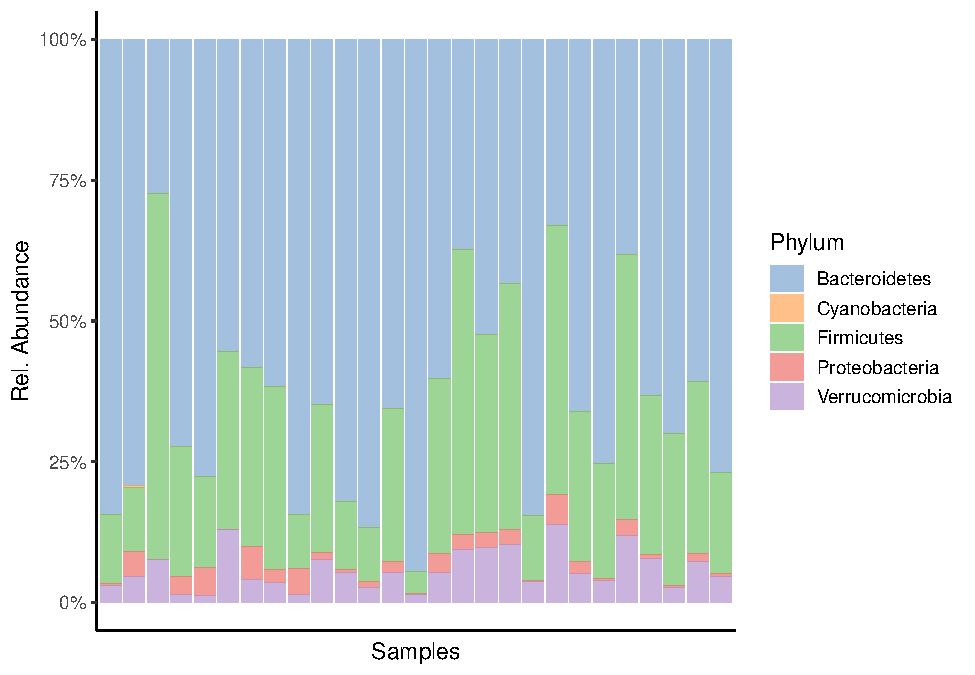
\includegraphics{radboud2021_material_files/figure-latex/unnamed-chunk-14-1.pdf}

\textbf{Density plot} shows the overall abundance distribution for a given
taxonomic group. Let us check the relative abundance of Firmicutes
across the sample collection. The density plot is a smoothened
version of a standard histogram.

The plot shows peak abundances around 30 \%.

\begin{Shaded}
\begin{Highlighting}[]
\CommentTok{\# Subset data by taking only Firmicutes}
\NormalTok{tse\_firmicutes }\OtherTok{\textless{}{-}}\NormalTok{ tse\_phylum[}\StringTok{"Firmicutes"}\NormalTok{]}

\CommentTok{\# Gets the abundance table}
\NormalTok{abundance\_firmicutes }\OtherTok{\textless{}{-}} \FunctionTok{assay}\NormalTok{(tse\_firmicutes, }\StringTok{"relabundance"}\NormalTok{)}

\CommentTok{\# Creates a data frame object, where first column includes abundances}
\NormalTok{firmicutes\_abund\_df }\OtherTok{\textless{}{-}} \FunctionTok{as.data.frame}\NormalTok{(}\FunctionTok{t}\NormalTok{(abundance\_firmicutes))}
\CommentTok{\# Rename the first and only column}
\FunctionTok{colnames}\NormalTok{(firmicutes\_abund\_df) }\OtherTok{\textless{}{-}} \StringTok{"abund"}

\CommentTok{\# Creates a plot. Parameters inside feom\_density are optional. With }
\CommentTok{\# geom\_density(bw=1000), it is possible to adjust bandwidth.}
\NormalTok{firmicutes\_abund\_plot }\OtherTok{\textless{}{-}} \FunctionTok{ggplot}\NormalTok{(firmicutes\_abund\_df, }\FunctionTok{aes}\NormalTok{(}\AttributeTok{x =}\NormalTok{ abund)) }\SpecialCharTok{+} 
  \FunctionTok{geom\_density}\NormalTok{(}\AttributeTok{color=}\StringTok{"darkred"}\NormalTok{, }\AttributeTok{fill=}\StringTok{"lightblue"}\NormalTok{) }\SpecialCharTok{+} 
  \FunctionTok{labs}\NormalTok{(}\AttributeTok{x =} \StringTok{"Relative abundance"}\NormalTok{, }\AttributeTok{title =} \StringTok{"Firmicutes"}\NormalTok{) }\SpecialCharTok{+}
  \FunctionTok{theme\_classic}\NormalTok{() }\SpecialCharTok{+} \CommentTok{\# Changes the background}
  \FunctionTok{scale\_x\_continuous}\NormalTok{(}\AttributeTok{label =}\NormalTok{ scales}\SpecialCharTok{::}\NormalTok{percent)}

\NormalTok{firmicutes\_abund\_plot}
\end{Highlighting}
\end{Shaded}

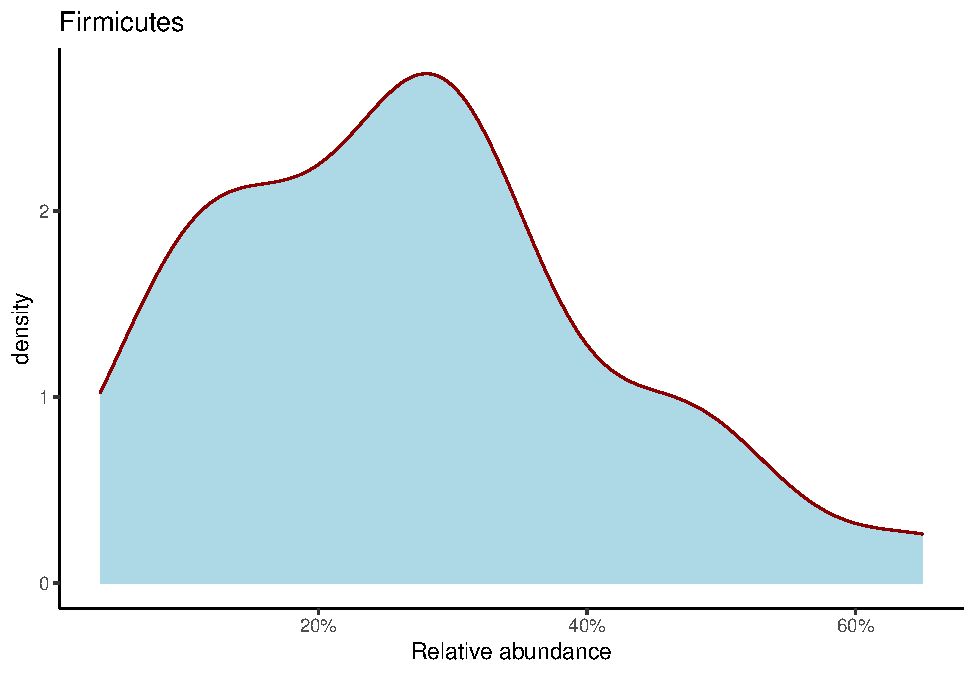
\includegraphics{radboud2021_material_files/figure-latex/unnamed-chunk-15-1.pdf}

For more visualization options and examples, see the \href{https://microbiome.github.io/miaViz/articles/miaViz.html}{miaViz vignette}.

\hypertarget{exercises-optional}{%
\section{Exercises (optional)}\label{exercises-optional}}

Explore some of the following questions on your own by following
\href{https://microbiome.github.io/OMA/}{online examples}. Prepare a
reproducible report (Rmarkdown), and include the code that you use to
import the data and generate the analyses.

\begin{itemize}
\item
  \textbf{Abundance table} Retrieve the taxonomic abundance table from the
  example data set (TSE object). Tip: check ``assays'' in \href{https://microbiome.github.io/OMA/data-introduction.html\#loading-experimental-microbiome-data}{data import
  section}
\item
  How many different samples and genus-level groups this phyloseq
  object has? Tips: see dim(), rowData()
\item
  What is the maximum abundance of Akkermansia in this data set? Tip:
  aggregate the data to Genus level with agglomerateByRank, pick
  abundance assay, and check a given genus (row) in the assay
\item
  Draw a histogram of library sizes (total number of reads per
  sample). Tip: Library size section in
  \href{https://microbiome.github.io/OMA/quality-control.html}{OMA}. You
  can use the available function, or count the sum of reads per
  sample by using the colSums command applied on the abundance
  table. Check \href{https://www.nature.com/articles/nature24460}{Vandeputte et
  al.~2017} for further
  discussion on the differences between absolute and relative
  quantification of microbial abundances.
\item
  \textbf{Taxonomy table} Retrieve the taxonomy table and print out the
  first few lines of it with the R command head(). Investigate how
  many different phylum-level groups this phyloseq object has? Tips:
  rowData, taxonomicRanks in
  \href{https://microbiome.github.io/OMA/taxonomic-information.html\#functions-to-access-taxonomic-information}{OMA}.
\item
  \textbf{Sample metadata} Retrieve sample metadata. How many patient
  groups this data set has? Draw a histogram of sample
  diversities. Tips: colData
\item
  \textbf{Subsetting} Pick a subset of the data object including only
  ADHD individuals from Cohort 1. How many there are? Tips: subsetSamples
\item
  \textbf{Transformations} The data contains read counts. We can convert
  these into relative abundances and other formats. Compare abundance
  of a given taxonomic group using the example data before and after
  the compositionality transformation (with a cross-plot, for
  instance). You can also compare the results to CLR-transformed data
  (see e.g.~\href{https://www.frontiersin.org/articles/10.3389/fmicb.2017.02224/full}{Gloor et
  al.~2017})
\item
  \textbf{Visual exploration} Visualize the population distribution of
  abundances for certain taxonomic groups. Do the same for
  CLR-transformed abundances. Tip: assays, transformCounts
\item
  Experiment with other data manipulation tools from
  \href{https://microbiome.github.io/OMA/taxonomic-information.html\#functions-to-access-taxonomic-information}{OMA}.
\item
  Example solution: \href{06-3-ex-sol-ADHD.html}{Solutions}
\end{itemize}

\hypertarget{alpha-diversity}{%
\chapter{Alpha diversity}\label{alpha-diversity}}

This section demonstrates the analysis of alpha diversity. This
quantity measures microbial diversity within each sample. Higher
numbers of unique taxa, and more even abundance distributions within a
sample yield larger values for alpha diversity.

Alpha diversity is a key quantity in a microbiome research. The \href{https://microbiome.github.io/mia/}{\emph{mia}
package} provides access to a wide
variety of alpha diversity indices. For more background information
and examples with various alpha diversity indices, see the \href{https://microbiome.github.io/OMA/microbiome-diversity.html\#alpha-diversity}{online
book}.

Let us show how to calculate to different diversity indices, Shannon
and Faith. Shannon index reflects how many different taxa there are
and how evenly they are distributed within a sample. Faith index
additionally takes into account the phylogenetic relations into
account.

\begin{Shaded}
\begin{Highlighting}[]
\CommentTok{\# Indices to be calculated. }
\CommentTok{\# Every index is calculated by default if we don\textquotesingle{}t specify indices.}
\NormalTok{indices }\OtherTok{\textless{}{-}} \FunctionTok{c}\NormalTok{(}\StringTok{"shannon"}\NormalTok{, }\StringTok{"faith"}\NormalTok{)}

\CommentTok{\# Indices are stored in colData (i.e., sample metadata). We can specify the name}
\CommentTok{\# of column, or we can use the default name which is the name of index }
\CommentTok{\# (i.e., "shannon" and "faith"). }
\NormalTok{names }\OtherTok{\textless{}{-}} \FunctionTok{c}\NormalTok{(}\StringTok{"Shannon\_diversity"}\NormalTok{, }\StringTok{"Faith\_diversity"}\NormalTok{)}

\CommentTok{\# Calculates indices}
\NormalTok{tse }\OtherTok{\textless{}{-}} \FunctionTok{estimateDiversity}\NormalTok{(tse, }\AttributeTok{index =}\NormalTok{ indices, }\AttributeTok{name =}\NormalTok{ names)}

\CommentTok{\# Shows the calculated indices}
\NormalTok{knitr}\SpecialCharTok{::}\FunctionTok{kable}\NormalTok{(}\FunctionTok{head}\NormalTok{(}\FunctionTok{colData}\NormalTok{(tse)[names])) }\SpecialCharTok{\%\textgreater{}\%} 
\NormalTok{  kableExtra}\SpecialCharTok{::}\FunctionTok{kable\_styling}\NormalTok{(}\StringTok{"striped"}\NormalTok{, }
                            \AttributeTok{latex\_options=}\StringTok{"scale\_down"}\NormalTok{) }\SpecialCharTok{\%\textgreater{}\%} 
\NormalTok{  kableExtra}\SpecialCharTok{::}\FunctionTok{scroll\_box}\NormalTok{(}\AttributeTok{width =} \StringTok{"100\%"}\NormalTok{)}
\end{Highlighting}
\end{Shaded}

\begin{table}
\centering
\resizebox{\linewidth}{!}{
\begin{tabular}{l|r|r}
\hline
  & Shannon\_diversity & Faith\_diversity\\
\hline
A110 & 1.765407 & 7.39224\\
\hline
A12 & 2.716438 & 6.29378\\
\hline
A15 & 3.178103 & 6.60608\\
\hline
A19 & 2.891987 & 6.79708\\
\hline
A21 & 2.841979 & 6.65110\\
\hline
A23 & 2.797942 & 5.96246\\
\hline
\end{tabular}}
\end{table}

Next we can visualize Shannon index with histogram.

\begin{Shaded}
\begin{Highlighting}[]
\CommentTok{\# ggplot needs data.frame format as input.}
\CommentTok{\# Here, colData is DataFrame, therefore it needs to be converted to data.frame}
\NormalTok{shannon\_hist }\OtherTok{\textless{}{-}} \FunctionTok{ggplot}\NormalTok{(}\FunctionTok{as.data.frame}\NormalTok{(}\FunctionTok{colData}\NormalTok{(tse)), }
                       \FunctionTok{aes}\NormalTok{(}\AttributeTok{x =}\NormalTok{ Shannon\_diversity)) }\SpecialCharTok{+} 
  \FunctionTok{geom\_histogram}\NormalTok{(}\AttributeTok{bins =} \DecValTok{20}\NormalTok{, }\AttributeTok{fill =} \StringTok{"gray"}\NormalTok{, }\AttributeTok{color =} \StringTok{"black"}\NormalTok{) }\SpecialCharTok{+}
  \FunctionTok{labs}\NormalTok{(}\AttributeTok{x =} \StringTok{"Shannon index"}\NormalTok{, }\AttributeTok{y =} \StringTok{"Sample frequency"}\NormalTok{)}

\NormalTok{shannon\_hist}
\end{Highlighting}
\end{Shaded}

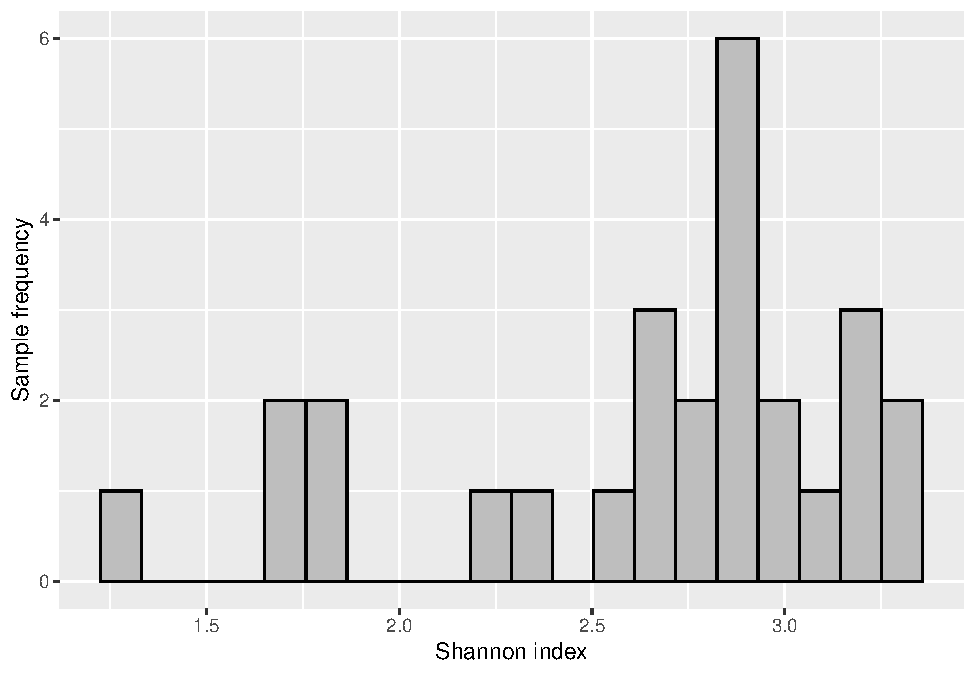
\includegraphics{radboud2021_material_files/figure-latex/unnamed-chunk-18-1.pdf}

Next, let us compare the indices based on a scatter-plot.

\begin{Shaded}
\begin{Highlighting}[]
\NormalTok{cross\_plot }\OtherTok{\textless{}{-}}\NormalTok{ ggplot2}\SpecialCharTok{::}\FunctionTok{ggplot}\NormalTok{(}\FunctionTok{as.data.frame}\NormalTok{(}\FunctionTok{colData}\NormalTok{(tse)), }
                                     \FunctionTok{aes}\NormalTok{(}\AttributeTok{x =}\NormalTok{ Shannon\_diversity, }\AttributeTok{y =}\NormalTok{ Faith\_diversity)) }\SpecialCharTok{+} 
  \FunctionTok{geom\_point}\NormalTok{() }\SpecialCharTok{+} \CommentTok{\# Adds points}
  \FunctionTok{geom\_smooth}\NormalTok{(}\AttributeTok{method=}\NormalTok{lm) }\SpecialCharTok{+} \CommentTok{\# Adds regression line}
  \FunctionTok{labs}\NormalTok{(}\AttributeTok{x =} \StringTok{"Shannon index"}\NormalTok{, }\AttributeTok{y =} \StringTok{"Faith diversity"}\NormalTok{) }

\NormalTok{cross\_plot}
\end{Highlighting}
\end{Shaded}

\begin{verbatim}
## `geom_smooth()` using formula 'y ~ x'
\end{verbatim}

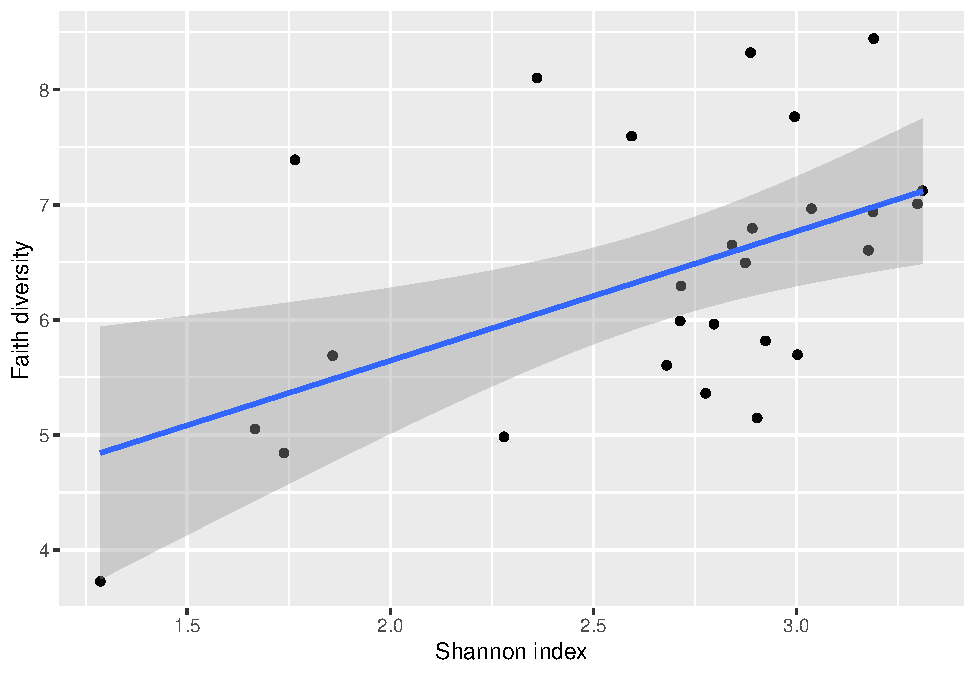
\includegraphics{radboud2021_material_files/figure-latex/unnamed-chunk-20-1.pdf}

\hypertarget{visualization-1}{%
\section{Visualization}\label{visualization-1}}

Next let us compare indices between different patient status and
cohorts. Boxplot is suitable for that purpose.

\begin{Shaded}
\begin{Highlighting}[]
\CommentTok{\# Creates Shannon boxplot }
\NormalTok{shannon\_box }\OtherTok{\textless{}{-}} \FunctionTok{ggplot}\NormalTok{(}\FunctionTok{as.data.frame}\NormalTok{(}\FunctionTok{colData}\NormalTok{(tse)),}
  \FunctionTok{aes}\NormalTok{(}\AttributeTok{x =}\NormalTok{ patient\_status, }
      \AttributeTok{y =}\NormalTok{ Shannon\_diversity,}
      \AttributeTok{fill =}\NormalTok{ cohort)) }\SpecialCharTok{+} 
  \FunctionTok{geom\_boxplot}\NormalTok{() }\SpecialCharTok{+}
  \FunctionTok{theme}\NormalTok{(}\AttributeTok{title =} \FunctionTok{element\_text}\NormalTok{(}\AttributeTok{size =} \DecValTok{12}\NormalTok{)) }\CommentTok{\# makes titles smaller}

\CommentTok{\# Creates Faith boxplot }
\NormalTok{faith\_box }\OtherTok{\textless{}{-}} \FunctionTok{ggplot}\NormalTok{(}\FunctionTok{as.data.frame}\NormalTok{(}\FunctionTok{colData}\NormalTok{(tse)), }\FunctionTok{aes}\NormalTok{(}\AttributeTok{x =}\NormalTok{ patient\_status, }
                                                     \AttributeTok{y =}\NormalTok{ Faith\_diversity, }
                                                     \AttributeTok{fill =}\NormalTok{ cohort)) }\SpecialCharTok{+} 
  \FunctionTok{geom\_boxplot}\NormalTok{() }\SpecialCharTok{+}
  \FunctionTok{theme}\NormalTok{(}\AttributeTok{title =} \FunctionTok{element\_text}\NormalTok{(}\AttributeTok{size =} \DecValTok{12}\NormalTok{)) }\CommentTok{\# makes titles smaller}

\CommentTok{\# Puts them into same picture}
\NormalTok{gridExtra}\SpecialCharTok{::}\FunctionTok{grid.arrange}\NormalTok{(shannon\_box, faith\_box, }\AttributeTok{nrow =} \DecValTok{2}\NormalTok{)}
\end{Highlighting}
\end{Shaded}

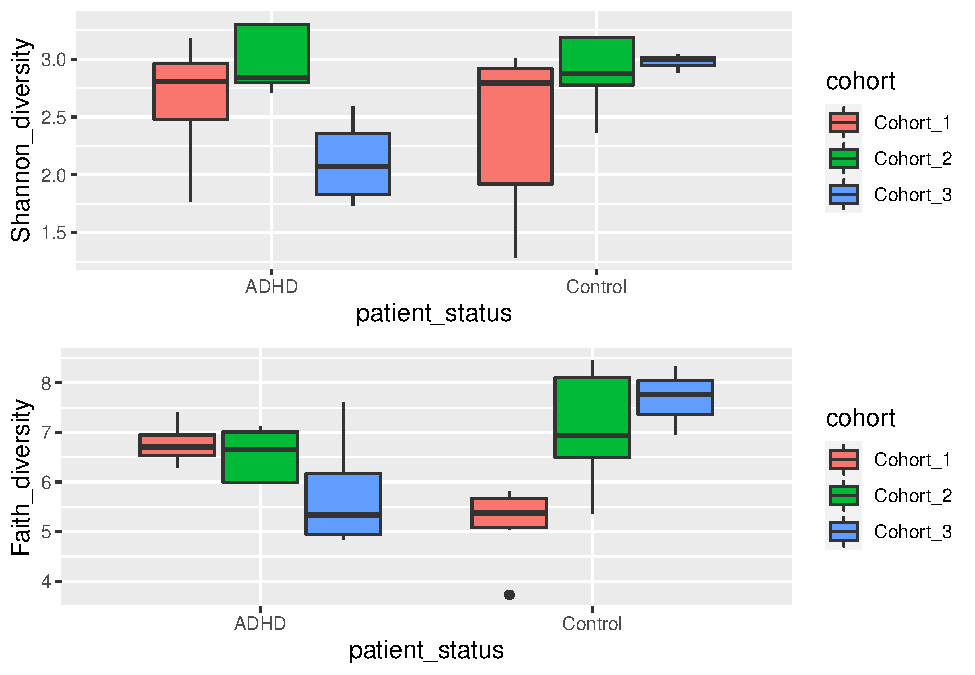
\includegraphics{radboud2021_material_files/figure-latex/unnamed-chunk-22-1.pdf}

For an alternative visualization, see examples with \href{https://microbiome.github.io/OMA/microbiome-diversity.html\#alpha-diversity}{scater::plotColData}.

\hypertarget{statistical-testing-and-comparisons}{%
\section{Statistical testing and comparisons}\label{statistical-testing-and-comparisons}}

To further investigate if patient status could explain the variation
of Shannon index, let's do a Wilcoxon test. This is a non-parametric
test that doesn't make specific assumptions about the distribution,
unlike popular parametric tests, such as the t test, which assumes
normally distributed observations.

Wilcoxon test can be used to estimate whether the differences between
two groups is statistically significant. Here the ADHD and control
groups are not significantly different between groups (p-value is over
0.05).

\begin{Shaded}
\begin{Highlighting}[]
\CommentTok{\# Wilcoxon test, where Shannon index is the variable that we are comparing. }
\CommentTok{\# Patient status {-} ADHD or control {-} is the factor that we use for grouping. }
\NormalTok{wilcoxon\_shannon }\OtherTok{\textless{}{-}} \FunctionTok{wilcox.test}\NormalTok{(Shannon\_diversity }\SpecialCharTok{\textasciitilde{}}\NormalTok{ patient\_status, }\AttributeTok{data =} \FunctionTok{colData}\NormalTok{(tse))}

\NormalTok{wilcoxon\_shannon}
\end{Highlighting}
\end{Shaded}

\begin{verbatim}
## 
##  Wilcoxon rank sum exact test
## 
## data:  Shannon_diversity by patient_status
## W = 76, p-value = 0.4879
## alternative hypothesis: true location shift is not equal to 0
\end{verbatim}

Another test that we can make is to test if ADHD samples differs between different
cohorts. From boxplot that we made in previous step, we can see that there might
be statistically significant difference between different cohorts.

Let's compare Shannon index of ADHD samples between cohort 2 and cohort 3.

As we can see, there is statistically significant difference between the cohorts.

\begin{Shaded}
\begin{Highlighting}[]
\CommentTok{\# Takes subset of colData. Takes only ADHD samples}
\NormalTok{ADHD\_shannon }\OtherTok{\textless{}{-}} \FunctionTok{colData}\NormalTok{(tse)[ }\FunctionTok{colData}\NormalTok{(tse)[, }\StringTok{"patient\_status"}\NormalTok{] }\SpecialCharTok{==} \StringTok{"ADHD"}\NormalTok{ , ]}

\CommentTok{\# Takes subset of colData. Takes only samples that are in cohort 2 or cohort 3.}
\NormalTok{ADHD\_shannon }\OtherTok{\textless{}{-}}\NormalTok{ ADHD\_shannon[ ADHD\_shannon[, }\StringTok{"cohort"}\NormalTok{] }\SpecialCharTok{\%in\%} \FunctionTok{c}\NormalTok{(}\StringTok{"Cohort\_2"}\NormalTok{, }\StringTok{"Cohort\_3"}\NormalTok{) , ]}

\CommentTok{\# Wilcoxon test, where Shannon index is the variable that we are comparing. }
\CommentTok{\# Cohort {-} 2 or 3 {-} is the factor that we use for grouping. }
\NormalTok{wilcoxon\_shannon\_ADHD\_cohorts }\OtherTok{\textless{}{-}} \FunctionTok{wilcox.test}\NormalTok{(Shannon\_diversity }\SpecialCharTok{\textasciitilde{}}\NormalTok{ cohort, }\AttributeTok{data =}\NormalTok{ ADHD\_shannon)}

\NormalTok{wilcoxon\_shannon\_ADHD\_cohorts}
\end{Highlighting}
\end{Shaded}

\begin{verbatim}
## 
##  Wilcoxon rank sum exact test
## 
## data:  Shannon_diversity by cohort
## W = 20, p-value = 0.01587
## alternative hypothesis: true location shift is not equal to 0
\end{verbatim}

For more examples, see a dedicated section on alpha diversity in the
\href{https://microbiome.github.io/OMA/microbiome-diversity.html\#alpha-diversity}{online book}.

\hypertarget{exercises}{%
\section{Exercises}\label{exercises}}

Add the following in the reproducible summary report.

\begin{itemize}
\item
  Estimate alpha diversity for each sample and draw a histogram. Tip:
  estimateDiversity
\item
  Compare the results between two or more
  alpha diversity indices (visually and/or statistically).
\item
  See \href{https://microbiome.github.io/OMA/microbiome-diversity.html\#alpha-diversity}{online book}
  for further examples.
\item
  Example \href{07-3-ex-sol-ADHD.html}{Solutions}
\end{itemize}

\hypertarget{beta-diversity}{%
\chapter{Beta diversity}\label{beta-diversity}}

Beta diversity is another name for sample dissimilarity. It quantifies
differences in the overall taxonomic composition between two samples.

Common indices include Bray-Curtis, Unifrac, Jaccard index, and the
Aitchison distance. Each of these (dis)similarity measures emphasizes
different aspects. For example, UniFrac incorporates phylogenetic
information, and Jaccard index ignores exact abundances and considers
only presence/absence values. For more background information
and examples, you can check the dedicated section in \href{https://microbiome.github.io/OMA/microbiome-diversity.html\#beta-diversity}{online
book}.

\hypertarget{examples-of-pcoa-with-different-settings}{%
\section{Examples of PCoA with different settings}\label{examples-of-pcoa-with-different-settings}}

Beta diversity estimation generates a (dis)similarity matrix that
contains for each sample (rows) the dissimilarity to any other sample
(columns).

This complex set of pairwise relations can be visualized in
informative ways, and even coupled with other explanatory
variables. As a first step, we compress the information to a lower
dimensionality, or fewer principal components, and then visualize
sample similarity based on that using ordination techniques, such as
Principal Coordinate Analysis (PCoA). PCoA is a non-linear dimension
reduction technique, and with Euclidean distances it is is identical
to the linear PCA (except for potential scaling).

We typically retain just the two (or three) most informative top
components, and ignore the other information. Each sample has a score
on each of these components, and each component measures the variation
across a set of correlated taxa. The top components are then easily
visualized on a two (or three) dimensional display.

Let us next look at some concrete examples.

\hypertarget{pcoa-for-asv-level-data-with-bray-curtis}{%
\subsection{PCoA for ASV-level data with Bray-Curtis}\label{pcoa-for-asv-level-data-with-bray-curtis}}

Let us start with PCoA based on a Bray-Curtis dissimilarity matrix
calculated at Genus level abundances.

\begin{Shaded}
\begin{Highlighting}[]
\CommentTok{\# Pick the relative abundance table}
\NormalTok{rel\_abund\_assay }\OtherTok{\textless{}{-}} \FunctionTok{assays}\NormalTok{(tse)}\SpecialCharTok{$}\NormalTok{relabundance}

\CommentTok{\# Calculates Bray{-}Curtis distances between samples. Because taxa is in}
\CommentTok{\# columns, it is used to compare different samples. We transpose the}
\CommentTok{\# assay to get taxa to columns}
\NormalTok{bray\_curtis\_dist }\OtherTok{\textless{}{-}}\NormalTok{ vegan}\SpecialCharTok{::}\FunctionTok{vegdist}\NormalTok{(}\FunctionTok{t}\NormalTok{(rel\_abund\_assay), }\AttributeTok{method =} \StringTok{"bray"}\NormalTok{)}

\CommentTok{\# PCoA}
\NormalTok{bray\_curtis\_pcoa }\OtherTok{\textless{}{-}}\NormalTok{ ecodist}\SpecialCharTok{::}\FunctionTok{pco}\NormalTok{(bray\_curtis\_dist)}

\CommentTok{\# All components could be found here: }
\CommentTok{\# bray\_curtis\_pcoa$vectors}
\CommentTok{\# But we only need the first two to demonstrate what we can do:}
\NormalTok{bray\_curtis\_pcoa\_df }\OtherTok{\textless{}{-}} \FunctionTok{data.frame}\NormalTok{(}\AttributeTok{pcoa1 =}\NormalTok{ bray\_curtis\_pcoa}\SpecialCharTok{$}\NormalTok{vectors[,}\DecValTok{1}\NormalTok{], }
                                  \AttributeTok{pcoa2 =}\NormalTok{ bray\_curtis\_pcoa}\SpecialCharTok{$}\NormalTok{vectors[,}\DecValTok{2}\NormalTok{])}

\CommentTok{\# Create a plot}
\NormalTok{bray\_curtis\_plot }\OtherTok{\textless{}{-}} \FunctionTok{ggplot}\NormalTok{(}\AttributeTok{data =}\NormalTok{ bray\_curtis\_pcoa\_df, }\FunctionTok{aes}\NormalTok{(}\AttributeTok{x=}\NormalTok{pcoa1, }\AttributeTok{y=}\NormalTok{pcoa2)) }\SpecialCharTok{+}
  \FunctionTok{geom\_point}\NormalTok{() }\SpecialCharTok{+}
  \FunctionTok{labs}\NormalTok{(}\AttributeTok{x =} \StringTok{"PC1"}\NormalTok{,}
       \AttributeTok{y =} \StringTok{"PC2"}\NormalTok{, }
       \AttributeTok{title =} \StringTok{"Bray{-}Curtis PCoA"}\NormalTok{) }\SpecialCharTok{+}
  \FunctionTok{theme}\NormalTok{(}\AttributeTok{title =} \FunctionTok{element\_text}\NormalTok{(}\AttributeTok{size =} \DecValTok{10}\NormalTok{)) }\CommentTok{\# makes titles smaller}

\NormalTok{bray\_curtis\_plot}
\end{Highlighting}
\end{Shaded}

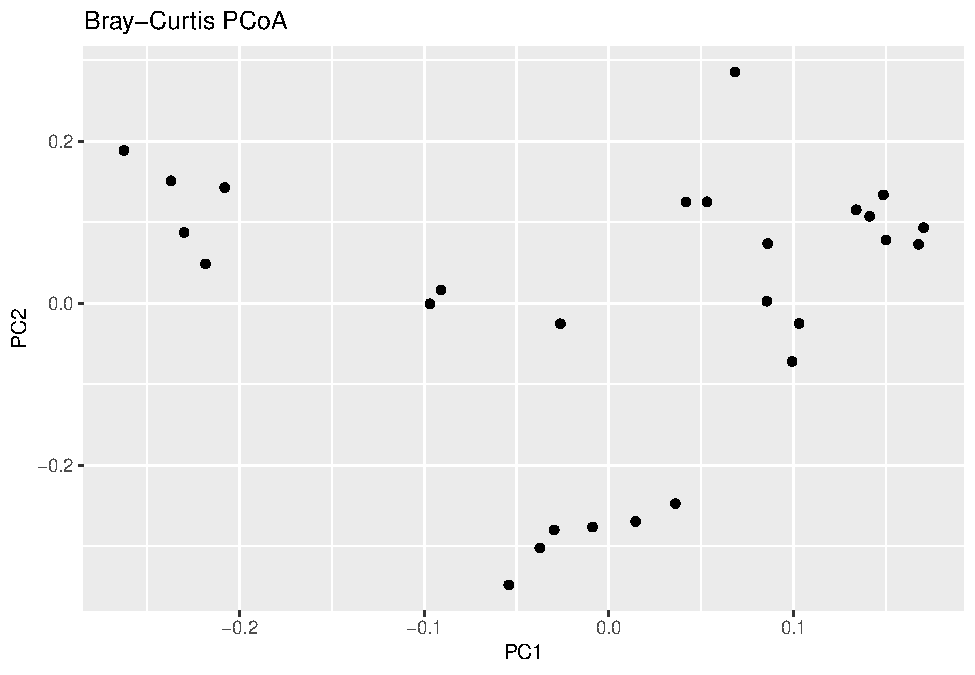
\includegraphics{radboud2021_material_files/figure-latex/pcoa_asv_bc-1.pdf}

\hypertarget{pcoa-for-asv-level-data-with-aitchison-distance}{%
\subsection{PCoA for ASV-level data with Aitchison distance}\label{pcoa-for-asv-level-data-with-aitchison-distance}}

Now the same using Aitchison distance. This metric corresponds to
Euclidean distances between CLR transformed sample abundance vectors.

\begin{Shaded}
\begin{Highlighting}[]
\CommentTok{\# Does clr transformation. Pseudocount is added, because data contains zeros. }
\NormalTok{tse }\OtherTok{\textless{}{-}} \FunctionTok{transformCounts}\NormalTok{(tse, }\AttributeTok{method =} \StringTok{"clr"}\NormalTok{, }\AttributeTok{pseudocount =} \DecValTok{1}\NormalTok{)}

\CommentTok{\# Gets clr table}
\NormalTok{clr\_assay }\OtherTok{\textless{}{-}} \FunctionTok{assays}\NormalTok{(tse)}\SpecialCharTok{$}\NormalTok{clr}

\CommentTok{\# Transposes it to get taxa to columns}
\NormalTok{clr\_assay }\OtherTok{\textless{}{-}} \FunctionTok{t}\NormalTok{(clr\_assay)}

\CommentTok{\# Calculates Euclidean distances between samples. Because taxa is in columns,}
\CommentTok{\# it is used to compare different samples.}
\NormalTok{euclidean\_dist }\OtherTok{\textless{}{-}}\NormalTok{ vegan}\SpecialCharTok{::}\FunctionTok{vegdist}\NormalTok{(clr\_assay, }\AttributeTok{method =} \StringTok{"euclidean"}\NormalTok{)}

\CommentTok{\# Does principal coordinate analysis}
\NormalTok{euclidean\_pcoa }\OtherTok{\textless{}{-}}\NormalTok{ ecodist}\SpecialCharTok{::}\FunctionTok{pco}\NormalTok{(euclidean\_dist)}

\CommentTok{\# Creates a data frame from principal coordinates}
\NormalTok{euclidean\_pcoa\_df }\OtherTok{\textless{}{-}} \FunctionTok{data.frame}\NormalTok{(}\AttributeTok{pcoa1 =}\NormalTok{ euclidean\_pcoa}\SpecialCharTok{$}\NormalTok{vectors[,}\DecValTok{1}\NormalTok{], }
                                \AttributeTok{pcoa2 =}\NormalTok{ euclidean\_pcoa}\SpecialCharTok{$}\NormalTok{vectors[,}\DecValTok{2}\NormalTok{])}

\CommentTok{\# Creates the plot}
\NormalTok{euclidean\_plot }\OtherTok{\textless{}{-}} \FunctionTok{ggplot}\NormalTok{(}\AttributeTok{data =}\NormalTok{ euclidean\_pcoa\_df, }\FunctionTok{aes}\NormalTok{(}\AttributeTok{x=}\NormalTok{pcoa1, }\AttributeTok{y=}\NormalTok{pcoa2)) }\SpecialCharTok{+}
  \FunctionTok{geom\_point}\NormalTok{() }\SpecialCharTok{+}
  \FunctionTok{labs}\NormalTok{(}\AttributeTok{x =} \StringTok{"PC1"}\NormalTok{,}
       \AttributeTok{y =} \StringTok{"PC22"}\NormalTok{,}
       \AttributeTok{title =} \StringTok{"Euclidean PCoA with CLR transformation"}\NormalTok{) }\SpecialCharTok{+}
  \FunctionTok{theme}\NormalTok{(}\AttributeTok{title =} \FunctionTok{element\_text}\NormalTok{(}\AttributeTok{size =} \DecValTok{12}\NormalTok{)) }\CommentTok{\# makes titles smaller}

\NormalTok{euclidean\_plot}
\end{Highlighting}
\end{Shaded}

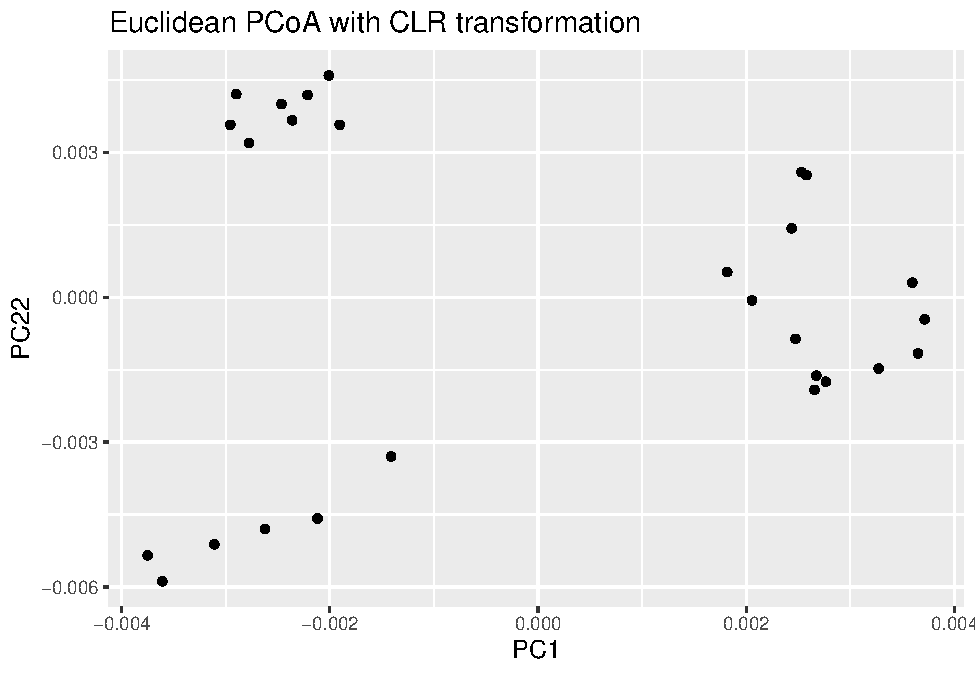
\includegraphics{radboud2021_material_files/figure-latex/pcoa_asv_aitchison-1.pdf}

\hypertarget{pcoa-aggregated-to-phylum-level}{%
\subsection{PCoA aggregated to Phylum level}\label{pcoa-aggregated-to-phylum-level}}

We use again the Aitchison distances in this example but this time applied to the phylum level.

\begin{Shaded}
\begin{Highlighting}[]
\CommentTok{\# Does clr transformation. Psuedocount is added, because data contains zeros. }
\NormalTok{tse\_phylum }\OtherTok{\textless{}{-}} \FunctionTok{transformCounts}\NormalTok{(tse\_phylum, }\AttributeTok{method =} \StringTok{"clr"}\NormalTok{, }\AttributeTok{pseudocount =} \DecValTok{1}\NormalTok{)}

\CommentTok{\# Gets clr table}
\NormalTok{clr\_phylum\_assay }\OtherTok{\textless{}{-}} \FunctionTok{assays}\NormalTok{(tse\_phylum)}\SpecialCharTok{$}\NormalTok{clr}

\CommentTok{\# Transposes it to get taxa to columns}
\NormalTok{clr\_phylum\_assay }\OtherTok{\textless{}{-}} \FunctionTok{t}\NormalTok{(clr\_phylum\_assay)}

\CommentTok{\# Calculates Euclidean distances between samples. Because taxa is in columns,}
\CommentTok{\# it is used to compare different samples.}
\NormalTok{euclidean\_phylum\_dist }\OtherTok{\textless{}{-}}\NormalTok{ vegan}\SpecialCharTok{::}\FunctionTok{vegdist}\NormalTok{(clr\_assay, }\AttributeTok{method =} \StringTok{"euclidean"}\NormalTok{)}

\CommentTok{\# Does principal coordinate analysis}
\NormalTok{euclidean\_phylum\_pcoa }\OtherTok{\textless{}{-}}\NormalTok{ ecodist}\SpecialCharTok{::}\FunctionTok{pco}\NormalTok{(euclidean\_phylum\_dist)}

\CommentTok{\# Creates a data frame from principal coordinates}
\NormalTok{euclidean\_phylum\_pcoa\_df }\OtherTok{\textless{}{-}} \FunctionTok{data.frame}\NormalTok{(}
  \AttributeTok{pcoa1 =}\NormalTok{ euclidean\_phylum\_pcoa}\SpecialCharTok{$}\NormalTok{vectors[,}\DecValTok{1}\NormalTok{], }
  \AttributeTok{pcoa2 =}\NormalTok{ euclidean\_phylum\_pcoa}\SpecialCharTok{$}\NormalTok{vectors[,}\DecValTok{2}\NormalTok{])}

\CommentTok{\# Creates a plot}
\NormalTok{euclidean\_phylum\_plot }\OtherTok{\textless{}{-}} \FunctionTok{ggplot}\NormalTok{(}\AttributeTok{data =}\NormalTok{ euclidean\_phylum\_pcoa\_df,}
  \FunctionTok{aes}\NormalTok{(}\AttributeTok{x=}\NormalTok{pcoa1, }\AttributeTok{y=}\NormalTok{pcoa2)) }\SpecialCharTok{+}
  \FunctionTok{geom\_point}\NormalTok{() }\SpecialCharTok{+}
  \FunctionTok{labs}\NormalTok{(}\AttributeTok{x =} \StringTok{"PC1"}\NormalTok{,}
       \AttributeTok{y =} \StringTok{"PC2"}\NormalTok{,}
       \AttributeTok{title =} \StringTok{"Aitchison distances at Phylum level"}\NormalTok{) }\SpecialCharTok{+}  
  \FunctionTok{theme}\NormalTok{(}\AttributeTok{title =} \FunctionTok{element\_text}\NormalTok{(}\AttributeTok{size =} \DecValTok{12}\NormalTok{)) }\CommentTok{\# makes titles smaller}

\NormalTok{euclidean\_phylum\_plot}
\end{Highlighting}
\end{Shaded}

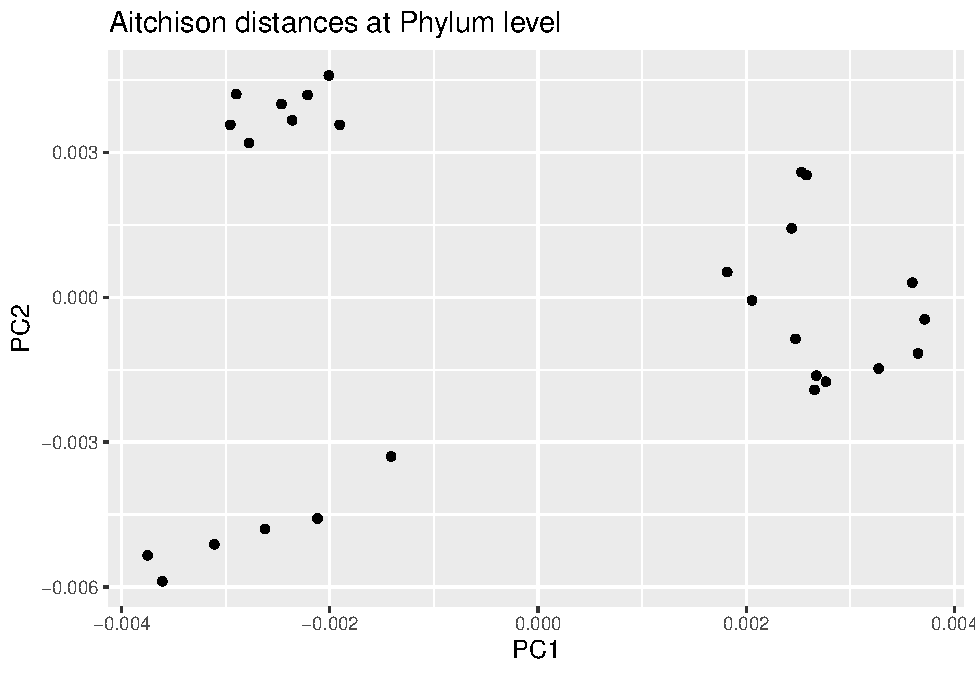
\includegraphics{radboud2021_material_files/figure-latex/pcoa_phylum_aitchison-1.pdf}

\hypertarget{highlighting-external-variables}{%
\section{Highlighting external variables}\label{highlighting-external-variables}}

We can map other variables on the same plot for example by coloring
the points accordingly.

\hypertarget{discrete-grouping-variable-shown-with-colors}{%
\subsection{Discrete grouping variable shown with colors}\label{discrete-grouping-variable-shown-with-colors}}

\begin{Shaded}
\begin{Highlighting}[]
\CommentTok{\# Adds the variable we later use for coloring to the data frame}
\NormalTok{euclidean\_patient\_status\_pcoa\_df }\OtherTok{\textless{}{-}} \FunctionTok{cbind}\NormalTok{(euclidean\_pcoa\_df,}
                             \AttributeTok{patient\_status =} \FunctionTok{colData}\NormalTok{(tse)}\SpecialCharTok{$}\NormalTok{patient\_status)}

\CommentTok{\# Creates a plot}
\NormalTok{euclidean\_patient\_status\_plot }\OtherTok{\textless{}{-}} \FunctionTok{ggplot}\NormalTok{(}\AttributeTok{data =}\NormalTok{ euclidean\_patient\_status\_pcoa\_df, }
                                        \FunctionTok{aes}\NormalTok{(}\AttributeTok{x=}\NormalTok{pcoa1, }\AttributeTok{y=}\NormalTok{pcoa2,}
                                            \AttributeTok{color =}\NormalTok{ patient\_status)) }\SpecialCharTok{+}
  \FunctionTok{geom\_point}\NormalTok{() }\SpecialCharTok{+}
  \FunctionTok{labs}\NormalTok{(}\AttributeTok{x =} \StringTok{"PC1"}\NormalTok{,}
       \AttributeTok{y =} \StringTok{"PC2"}\NormalTok{,}
       \AttributeTok{title =} \StringTok{"PCoA with Aitchison distances"}\NormalTok{) }\SpecialCharTok{+}
  \FunctionTok{theme}\NormalTok{(}\AttributeTok{title =} \FunctionTok{element\_text}\NormalTok{(}\AttributeTok{size =} \DecValTok{12}\NormalTok{)) }\CommentTok{\# makes titles smaller}

\NormalTok{euclidean\_patient\_status\_plot}
\end{Highlighting}
\end{Shaded}

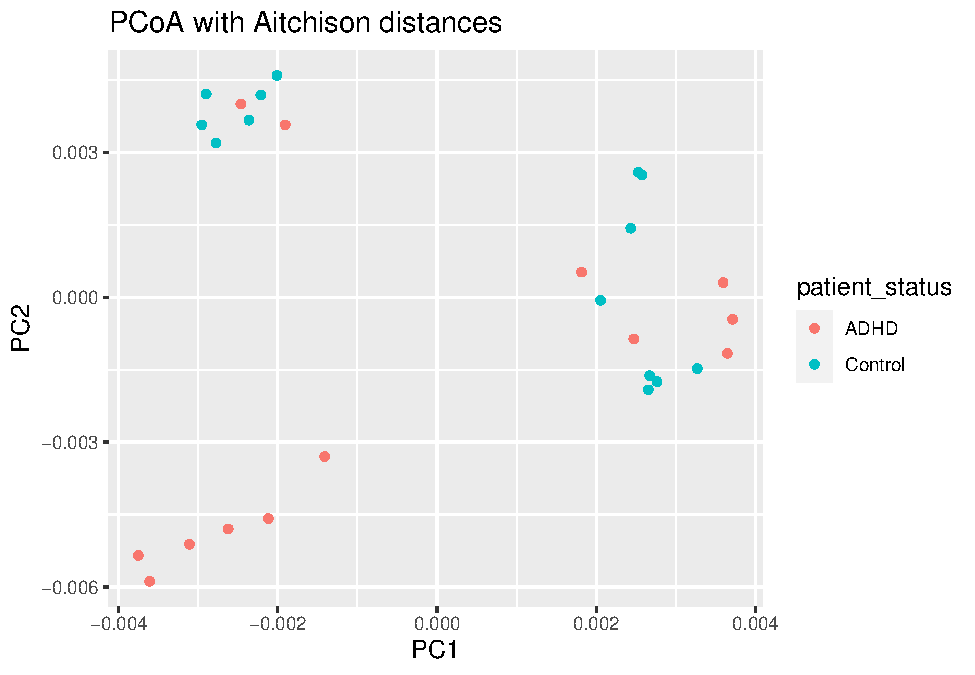
\includegraphics{radboud2021_material_files/figure-latex/pcoa_genus-1.pdf}

\hypertarget{pcoa-plot-with-continuous-variable}{%
\subsection{PCoA plot with continuous variable}\label{pcoa-plot-with-continuous-variable}}

We can do the same as above using any continuous variable. E.g. let us
see how the plotted samples differ in their alpha diversity (as an
example of a continuous variable):

\begin{Shaded}
\begin{Highlighting}[]
\CommentTok{\# Adds coloring information to the data frame, creates new column}
\NormalTok{euclidean\_shannon\_pcoa\_df }\OtherTok{\textless{}{-}} \FunctionTok{cbind}\NormalTok{(euclidean\_pcoa\_df,}
                             \AttributeTok{shannon =} \FunctionTok{colData}\NormalTok{(tse)}\SpecialCharTok{$}\NormalTok{Shannon\_diversity)}

\CommentTok{\# Creates a plot}
\NormalTok{euclidean\_shannon\_plot }\OtherTok{\textless{}{-}} \FunctionTok{ggplot}\NormalTok{(}\AttributeTok{data =}\NormalTok{ euclidean\_shannon\_pcoa\_df, }
                                 \FunctionTok{aes}\NormalTok{(}\AttributeTok{x=}\NormalTok{pcoa1, }\AttributeTok{y=}\NormalTok{pcoa2,}
                                     \AttributeTok{color =}\NormalTok{ shannon)) }\SpecialCharTok{+} 
  \FunctionTok{geom\_point}\NormalTok{() }\SpecialCharTok{+}
  \FunctionTok{labs}\NormalTok{(}\AttributeTok{x =} \StringTok{"PC1"}\NormalTok{,}
       \AttributeTok{y =} \StringTok{"PC2"}\NormalTok{,}
       \AttributeTok{title =} \StringTok{"PCoA with Aitchison distances"}\NormalTok{) }\SpecialCharTok{+}
  \FunctionTok{theme}\NormalTok{(}\AttributeTok{title =} \FunctionTok{element\_text}\NormalTok{(}\AttributeTok{size =} \DecValTok{12}\NormalTok{)) }\CommentTok{\# makes titles smaller}

\NormalTok{euclidean\_shannon\_plot}
\end{Highlighting}
\end{Shaded}

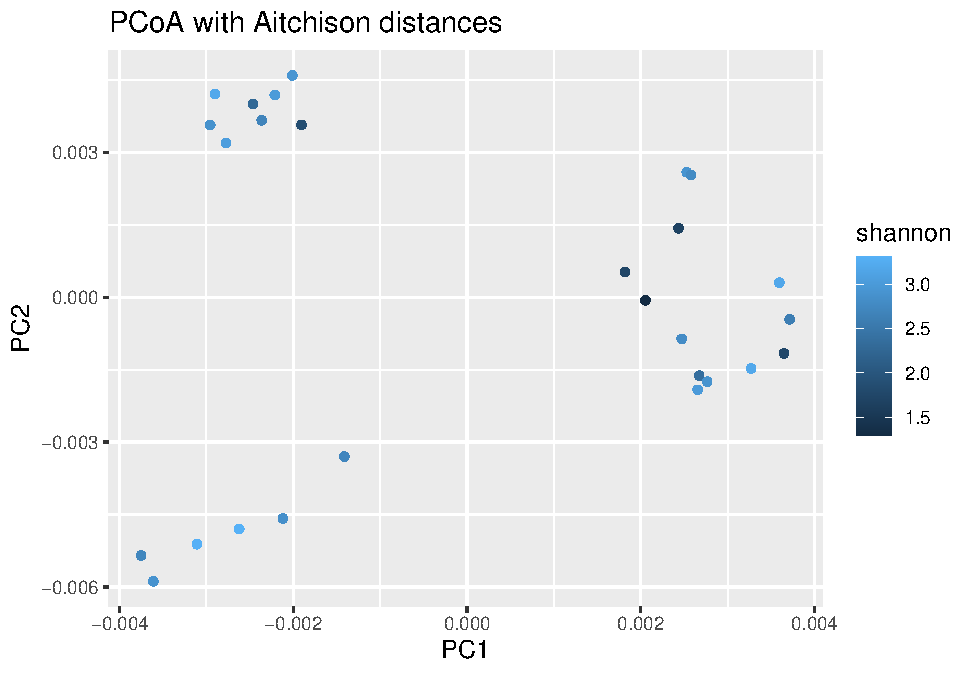
\includegraphics{radboud2021_material_files/figure-latex/pcoa_coloring-1.pdf}

\hypertarget{estimating-associations-with-an-external-variable}{%
\section{Estimating associations with an external variable}\label{estimating-associations-with-an-external-variable}}

Next to visualizing whether any variable is associated with
differences between samples, we can also quantify the strength of the
association between community composition (beta diversity) and
external factors.

The standard way to do this is to perform a so-called permutational
multivariate analysis of variance (PERMANOVA). This method takes as
input the abundance table, which measure of distance you want to base
the test on and a formula that tells the model how you think the
variables are associated with each other.

\begin{Shaded}
\begin{Highlighting}[]
\CommentTok{\# First we get the relative abundance table}
\NormalTok{rel\_abund\_assay }\OtherTok{\textless{}{-}} \FunctionTok{assays}\NormalTok{(tse)}\SpecialCharTok{$}\NormalTok{relabundance}

\CommentTok{\# again transpose it to get taxa to columns}
\NormalTok{rel\_abund\_assay }\OtherTok{\textless{}{-}} \FunctionTok{t}\NormalTok{(rel\_abund\_assay)}

\CommentTok{\# then we can perform the method}
\NormalTok{permanova\_cohort }\OtherTok{\textless{}{-}}\NormalTok{ vegan}\SpecialCharTok{::}\FunctionTok{adonis}\NormalTok{(rel\_abund\_assay }\SpecialCharTok{\textasciitilde{}}\NormalTok{ cohort,}
                                  \AttributeTok{data =} \FunctionTok{colData}\NormalTok{(tse),}
                                  \AttributeTok{permutations =} \DecValTok{9999}\NormalTok{)}

\CommentTok{\# we can obtain a the p value for our predictor:}
\FunctionTok{print}\NormalTok{(}\FunctionTok{paste0}\NormalTok{(}\StringTok{"Different different cohorts and variance of abundance "}\NormalTok{,}
              \StringTok{"between samples, p{-}value: "}\NormalTok{, }
              \FunctionTok{as.data.frame}\NormalTok{(permanova\_cohort}\SpecialCharTok{$}\NormalTok{aov.tab)[}\StringTok{"cohort"}\NormalTok{, }\StringTok{"Pr(\textgreater{}F)"}\NormalTok{]))}
\end{Highlighting}
\end{Shaded}

\begin{verbatim}
## [1] "Different different cohorts and variance of abundance between samples, p-value: 0.7395"
\end{verbatim}

The cohort variable is not significantly associated with
microbiota composition (p-value is over 0.05).

We can, however, visualize those taxa whose abundances drive the
differences between cohorts. We first need to extract the model
coefficients of taxa:

\begin{Shaded}
\begin{Highlighting}[]
\CommentTok{\# Gets the coefficients}
\NormalTok{coef }\OtherTok{\textless{}{-}} \FunctionTok{coefficients}\NormalTok{(permanova\_cohort)[}\StringTok{"cohort1"}\NormalTok{,]}

\CommentTok{\# Gets the highest coefficients}
\NormalTok{top.coef }\OtherTok{\textless{}{-}} \FunctionTok{sort}\NormalTok{(}\FunctionTok{head}\NormalTok{(coef[}\FunctionTok{rev}\NormalTok{(}\FunctionTok{order}\NormalTok{(}\FunctionTok{abs}\NormalTok{(coef)))],}\DecValTok{20}\NormalTok{))}

\CommentTok{\# Plots the coefficients}
\NormalTok{top\_taxa\_coeffient\_plot }\OtherTok{\textless{}{-}} \FunctionTok{ggplot}\NormalTok{(}\FunctionTok{data.frame}\NormalTok{(}\AttributeTok{x =}\NormalTok{ top.coef,}
                                             \AttributeTok{y =} \FunctionTok{factor}\NormalTok{(}\FunctionTok{names}\NormalTok{(top.coef),}
                         \FunctionTok{unique}\NormalTok{(}\FunctionTok{names}\NormalTok{(top.coef)))),}
                                  \FunctionTok{aes}\NormalTok{(}\AttributeTok{x =}\NormalTok{ x, }\AttributeTok{y =}\NormalTok{ y)) }\SpecialCharTok{+}
  \FunctionTok{geom\_bar}\NormalTok{(}\AttributeTok{stat=}\StringTok{"identity"}\NormalTok{) }\SpecialCharTok{+}
  \FunctionTok{labs}\NormalTok{(}\AttributeTok{x=}\StringTok{""}\NormalTok{, }\AttributeTok{y=}\StringTok{""}\NormalTok{, }\AttributeTok{title=}\StringTok{"Top Taxa"}\NormalTok{) }\SpecialCharTok{+}
  \FunctionTok{theme\_bw}\NormalTok{()}

\NormalTok{top\_taxa\_coeffient\_plot}
\end{Highlighting}
\end{Shaded}

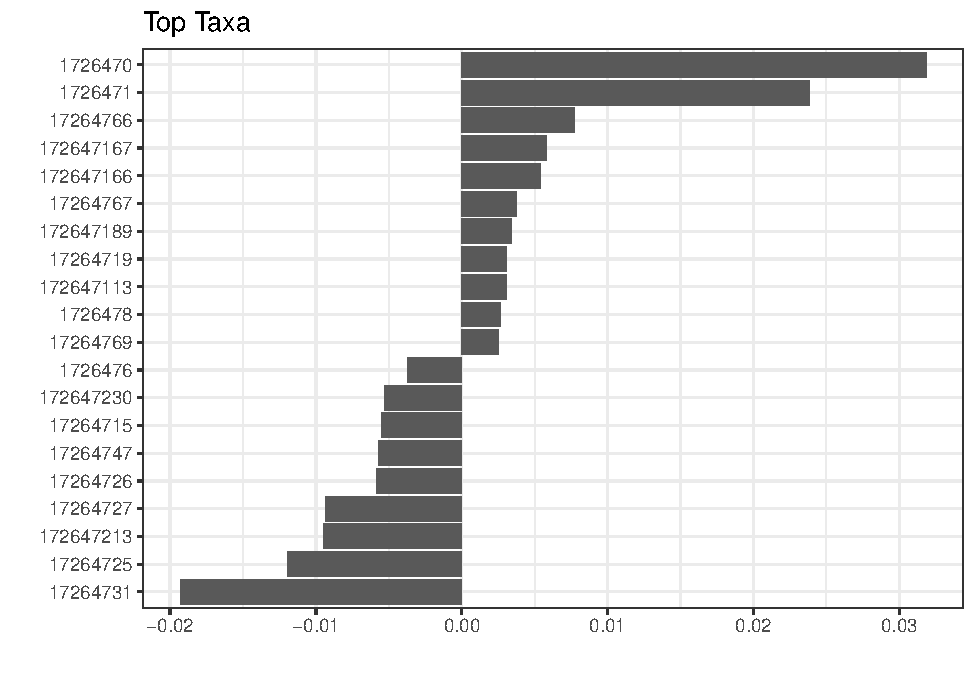
\includegraphics{radboud2021_material_files/figure-latex/permanova_coefs-1.pdf}

The above plot shows taxa as code names, and it is hard to tell which
bacterial groups they represent. However, it is easy to add human readable
names. We can fetch those from our rowData. Here we use Genus level names:

\begin{Shaded}
\begin{Highlighting}[]
\CommentTok{\# Gets corresponding Genus level names and stores them to top.coef}
\NormalTok{names }\OtherTok{\textless{}{-}} \FunctionTok{rowData}\NormalTok{(tse)[}\FunctionTok{names}\NormalTok{(top.coef), ][,}\StringTok{"Genus"}\NormalTok{]}

\CommentTok{\# Adds new labels to the plot}
\NormalTok{top\_taxa\_coeffient\_plot }\OtherTok{\textless{}{-}}\NormalTok{ top\_taxa\_coeffient\_plot }\SpecialCharTok{+}
  \FunctionTok{scale\_y\_discrete}\NormalTok{(}\AttributeTok{labels =}\NormalTok{ names) }\CommentTok{\# Adds new labels}
\NormalTok{top\_taxa\_coeffient\_plot}
\end{Highlighting}
\end{Shaded}

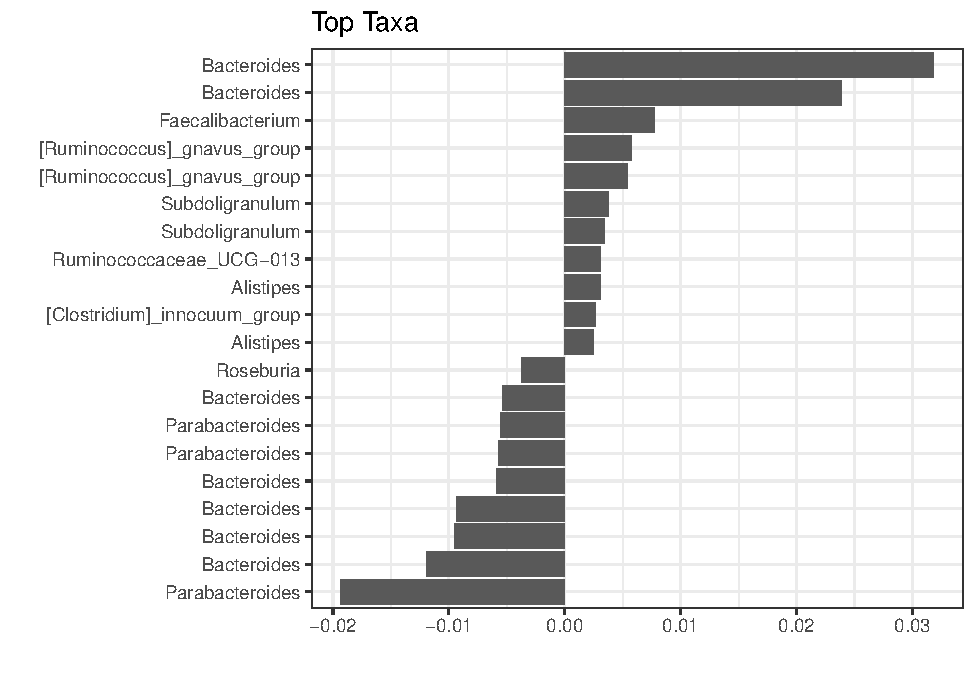
\includegraphics{radboud2021_material_files/figure-latex/unnamed-chunk-25-1.pdf}

There are many alternative and complementary methods for analysing
community composition. For more examples, see a dedicated section on
beta diversity in the \href{https://microbiome.github.io/OMA/microbiome-diversity.html\#beta-diversity}{online
book}.

\hypertarget{community-typing}{%
\section{Community typing}\label{community-typing}}

A dedicated section presenting examples on community typing is in the
\href{https://microbiome.github.io/OMA/microbiome-community.html\#community-typing}{online book}.

\hypertarget{exercises-1}{%
\section{Exercises}\label{exercises-1}}

\begin{itemize}
\item
  Visualize community variation with different methods (PCA, MDS, t-SNE\ldots) by using the options in the alternative method, plotReducedDim \href{https://microbiome.github.io/OMA/microbiome-diversity.html\#estimating-beta-diversity}{OMA}. Compare results obtained with different dissimilarities (Euclidean, Bray-Curtis, Unifrac..) and transformations (CLR, compositional..) of your own choice."
\item
  Investigate the influence of the data transformations on
  statistical analysis: Visualize community variation with PCoA with
  the following options: 1) Bray-Curtis distances for compositional
  data; 2) Euclidean distances for CLR-transformed data.
\item
  Community-level comparisons: Use PERMANOVA to investigate whether
  the community composition differs between two groups of individuals
  (e.g.~males and females, or some other grouping of your
  choice). You can also include covariates such as age and gender,
  and see how this affects the results.
\item
  Perform community typing for the data using the DMM method \href{https://microbiome.github.io/OMA/microbiome-community.html\#community-typing}{OMA}
\item
  Example \href{08-5-ex-sol-ADHD.html}{Solutions}
\end{itemize}

\hypertarget{differential-abundance-analysis}{%
\chapter{Differential abundance analysis}\label{differential-abundance-analysis}}

Here, we analyse abundances with three different methods: \textbf{Wilcoxon test}, \textbf{DESeq2},
and \textbf{ANCOM-BC}. All of these test statistical differences between groups.
We analyse Genus level abundances.

\hypertarget{wilcoxon-test}{%
\section{Wilcoxon test}\label{wilcoxon-test}}

A Wilcoxon test estimates difference between two groups. It is a
non-parametric alternative to a t-test, which means that the Wilcoxon test
does not require normally distributed data.

Let's first collect the data for the testing purpose.

\begin{Shaded}
\begin{Highlighting}[]
\CommentTok{\# Agglomerates data to Genus level}
\NormalTok{tse\_genus }\OtherTok{\textless{}{-}} \FunctionTok{agglomerateByRank}\NormalTok{(tse, }\AttributeTok{rank =} \StringTok{"Genus"}\NormalTok{)}

\CommentTok{\# Does clr transformation. Pseudocount is added, because data contains zeros, and}
\CommentTok{\# clr transformation includes log transformation.}
\NormalTok{tse\_genus }\OtherTok{\textless{}{-}} \FunctionTok{transformCounts}\NormalTok{(tse\_genus, }\AttributeTok{method =} \StringTok{"clr"}\NormalTok{, }\AttributeTok{pseudocount =} \DecValTok{1}\NormalTok{)}

\CommentTok{\# Does transpose, so samples are in rows, then creates a data frame.}
\NormalTok{abundance\_analysis\_data }\OtherTok{\textless{}{-}} \FunctionTok{data.frame}\NormalTok{(}\FunctionTok{t}\NormalTok{(}\FunctionTok{assay}\NormalTok{(tse\_genus, }\StringTok{"clr"}\NormalTok{)))}

\CommentTok{\# Then we need variable for grouping samples. "patient\_status" column includes information}
\CommentTok{\# about patients\textquotesingle{} status. There two groups "ADHD" and "control". }
\CommentTok{\# Let\textquotesingle{}s include that to the data frame.}
\NormalTok{abundance\_analysis\_data }\OtherTok{\textless{}{-}} \FunctionTok{cbind}\NormalTok{(abundance\_analysis\_data, }
                                 \AttributeTok{patient\_status =} \FunctionTok{colData}\NormalTok{(tse\_genus)}\SpecialCharTok{$}\NormalTok{patient\_status)}
\end{Highlighting}
\end{Shaded}

Now we can do the Wilcoxon test. We test all the taxa by looping through columns,
and store individual p-values to a vector. Then we create a data frame from collected
data.

Code below does the Wilcoxon test only for columns that contain abundances,
not for column that contain patient status.

\begin{Shaded}
\begin{Highlighting}[]
\NormalTok{colnames }\OtherTok{\textless{}{-}} \FunctionTok{names}\NormalTok{(abundance\_analysis\_data[, }\SpecialCharTok{!}\FunctionTok{names}\NormalTok{(abundance\_analysis\_data) }\SpecialCharTok{\%in\%} 
                                            \StringTok{"patient\_status"}\NormalTok{])}

\NormalTok{wilcoxon\_p }\OtherTok{\textless{}{-}} \FunctionTok{c}\NormalTok{() }\CommentTok{\# Initialize empty vector for p{-}values}

\CommentTok{\# Do for loop over selected column names}
\ControlFlowTok{for}\NormalTok{ (i }\ControlFlowTok{in}\NormalTok{ colnames) \{}

\NormalTok{  result }\OtherTok{\textless{}{-}} \FunctionTok{wilcox.test}\NormalTok{(abundance\_analysis\_data[, i] }\SpecialCharTok{\textasciitilde{}}\NormalTok{ patient\_status,}
                        \AttributeTok{data =}\NormalTok{ abundance\_analysis\_data)}
  
  \CommentTok{\# Stores p{-}value to the vector with this column name}
\NormalTok{  wilcoxon\_p[[i]]  }\OtherTok{\textless{}{-}}\NormalTok{ result}\SpecialCharTok{$}\NormalTok{p.value}

\NormalTok{\}}

\NormalTok{wilcoxon\_p }\OtherTok{\textless{}{-}} \FunctionTok{data.frame}\NormalTok{(}\AttributeTok{taxa =}  \FunctionTok{names}\NormalTok{(wilcoxon\_p),}
                         \AttributeTok{p\_raw =} \FunctionTok{unlist}\NormalTok{(wilcoxon\_p))}
\end{Highlighting}
\end{Shaded}

Multiple tests were performed. These are not independent, so we need
to adjust p-values for multiple testing. Otherwise, we would increase
the chance of a type I error drastically depending on our p-value
threshold. By applying a p-value adjustment, we can keep the false
positive rate at a level that is acceptable. What is acceptable
depends on our research goals. Here we use the fdr method, but there
are several other methods as well.

\begin{Shaded}
\begin{Highlighting}[]
\NormalTok{wilcoxon\_p}\SpecialCharTok{$}\NormalTok{p\_adjusted }\OtherTok{\textless{}{-}} \FunctionTok{p.adjust}\NormalTok{(wilcoxon\_p}\SpecialCharTok{$}\NormalTok{p\_raw, }\AttributeTok{method =} \StringTok{"fdr"}\NormalTok{)}
\end{Highlighting}
\end{Shaded}

\begin{Shaded}
\begin{Highlighting}[]
\NormalTok{df }\OtherTok{\textless{}{-}} \FunctionTok{data.frame}\NormalTok{(}\AttributeTok{x =} \FunctionTok{c}\NormalTok{(wilcoxon\_p}\SpecialCharTok{$}\NormalTok{p\_raw, wilcoxon\_p}\SpecialCharTok{$}\NormalTok{p\_adjusted), }
                \AttributeTok{type=}\FunctionTok{rep}\NormalTok{(}\FunctionTok{c}\NormalTok{(}\StringTok{"raw"}\NormalTok{, }\StringTok{"holm"}\NormalTok{),}
        \FunctionTok{c}\NormalTok{(}\FunctionTok{length}\NormalTok{(wilcoxon\_p}\SpecialCharTok{$}\NormalTok{p\_raw),}
          \FunctionTok{length}\NormalTok{(wilcoxon\_p}\SpecialCharTok{$}\NormalTok{p\_adjusted))))}

\NormalTok{wilcoxon\_plot }\OtherTok{\textless{}{-}} \FunctionTok{ggplot}\NormalTok{(df) }\SpecialCharTok{+}
  \FunctionTok{geom\_histogram}\NormalTok{(}\FunctionTok{aes}\NormalTok{(}\AttributeTok{x=}\NormalTok{x, }\AttributeTok{fill=}\NormalTok{type)) }\SpecialCharTok{+}
  \FunctionTok{labs}\NormalTok{(}\AttributeTok{x =} \StringTok{"p{-}value"}\NormalTok{, }\AttributeTok{y =} \StringTok{"Frequency"}\NormalTok{) }

\NormalTok{wilcoxon\_plot}
\end{Highlighting}
\end{Shaded}

\begin{verbatim}
## `stat_bin()` using `bins = 30`. Pick better value with `binwidth`.
\end{verbatim}

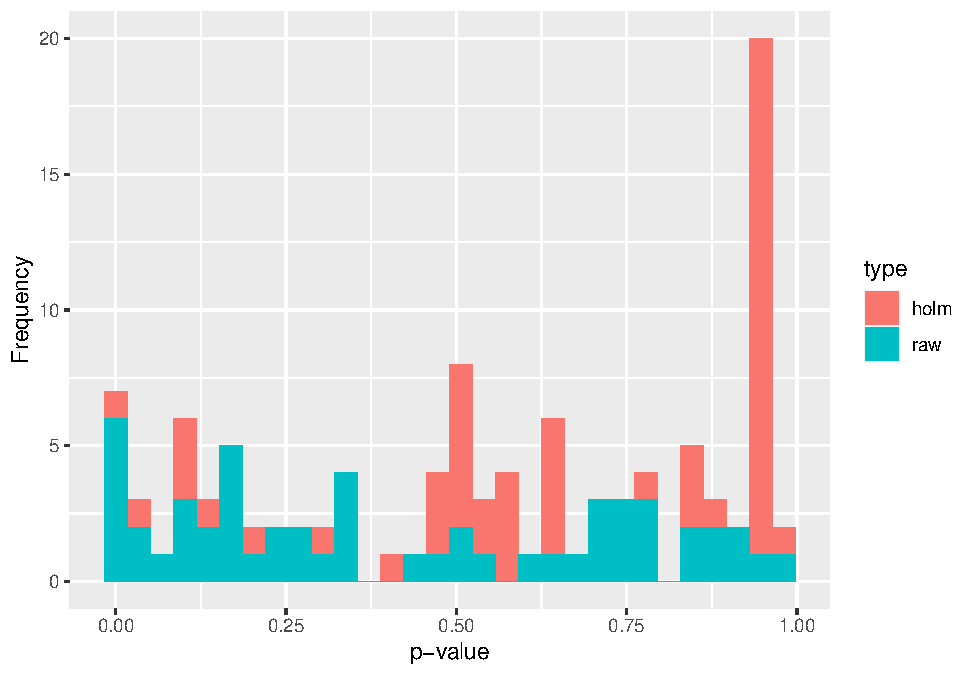
\includegraphics{radboud2021_material_files/figure-latex/unnamed-chunk-29-1.pdf}

\hypertarget{deseq2}{%
\section{DESeq2}\label{deseq2}}

Our second analysis method is DESeq2. This performs the data
normalization automatically. It also takes care of the p-value
adjustment, so we don't have to worry about that.

DESeq2 uses negative binomial distribution to detect differences in
read counts between groups. Its normalization takes care of the
differences between library sizes and compositions. DESeq2 analysis
includes multiple steps, but they are done automatically. More
information can be found, e.g., from Harvard Chan Bioinformatic Core's
tutorial \href{https://hbctraining.github.io/DGE_workshop/lessons/04_DGE_DESeq2_analysis.html}{Introduction to DGE -
ARCHIVED}

Now let us show how to do this. First, run the DESeq2 analysis.

\begin{Shaded}
\begin{Highlighting}[]
\CommentTok{\# Creates DESeq2 object from the data. Uses "patient\_status" to create groups. }
\NormalTok{ds2 }\OtherTok{\textless{}{-}} \FunctionTok{DESeqDataSet}\NormalTok{(tse\_genus, }\SpecialCharTok{\textasciitilde{}}\NormalTok{patient\_status)}
\end{Highlighting}
\end{Shaded}

\begin{verbatim}
## converting counts to integer mode
\end{verbatim}

\begin{verbatim}
## Warning in DESeqDataSet(tse_genus, ~patient_status): 2 duplicate rownames were renamed by adding numbers
\end{verbatim}

\begin{verbatim}
## Warning in DESeqDataSet(tse_genus, ~patient_status): some variables in design formula are characters, converting to factors
\end{verbatim}

\begin{Shaded}
\begin{Highlighting}[]
\CommentTok{\# Does the analysis}
\NormalTok{dds }\OtherTok{\textless{}{-}} \FunctionTok{DESeq}\NormalTok{(ds2)}
\end{Highlighting}
\end{Shaded}

\begin{verbatim}
## estimating size factors
\end{verbatim}

\begin{verbatim}
## estimating dispersions
\end{verbatim}

\begin{verbatim}
## gene-wise dispersion estimates
\end{verbatim}

\begin{verbatim}
## mean-dispersion relationship
\end{verbatim}

\begin{verbatim}
## final dispersion estimates
\end{verbatim}

\begin{verbatim}
## fitting model and testing
\end{verbatim}

\begin{verbatim}
## -- replacing outliers and refitting for 11 genes
## -- DESeq argument 'minReplicatesForReplace' = 7 
## -- original counts are preserved in counts(dds)
\end{verbatim}

\begin{verbatim}
## estimating dispersions
\end{verbatim}

\begin{verbatim}
## fitting model and testing
\end{verbatim}

\begin{Shaded}
\begin{Highlighting}[]
\CommentTok{\# Gets the results from the object}
\NormalTok{res }\OtherTok{\textless{}{-}} \FunctionTok{results}\NormalTok{(dds)}

\CommentTok{\# Creates a data frame from results}
\NormalTok{df }\OtherTok{\textless{}{-}} \FunctionTok{as.data.frame}\NormalTok{(res)}

\CommentTok{\# Adds taxon column that includes names of taxa}
\NormalTok{df}\SpecialCharTok{$}\NormalTok{taxon }\OtherTok{\textless{}{-}} \FunctionTok{rownames}\NormalTok{(df)}

\CommentTok{\# Orders the rows of data frame in increasing order firstly based on }
\CommentTok{\# column "log2FoldChange" and secondly based on "padj" column}
\NormalTok{df }\OtherTok{\textless{}{-}}\NormalTok{ df }\SpecialCharTok{\%\textgreater{}\%} \FunctionTok{arrange}\NormalTok{(log2FoldChange, padj)}

\NormalTok{knitr}\SpecialCharTok{::}\FunctionTok{kable}\NormalTok{(}\FunctionTok{head}\NormalTok{(df)) }\SpecialCharTok{\%\textgreater{}\%} 
\NormalTok{  kableExtra}\SpecialCharTok{::}\FunctionTok{kable\_styling}\NormalTok{(}\StringTok{"striped"}\NormalTok{, }
                            \AttributeTok{latex\_options=}\StringTok{"scale\_down"}\NormalTok{) }\SpecialCharTok{\%\textgreater{}\%} 
\NormalTok{  kableExtra}\SpecialCharTok{::}\FunctionTok{scroll\_box}\NormalTok{(}\AttributeTok{width =} \StringTok{"100\%"}\NormalTok{)}
\end{Highlighting}
\end{Shaded}

\begin{table}
\centering
\resizebox{\linewidth}{!}{
\begin{tabular}{l|r|r|r|r|r|r|l}
\hline
  & baseMean & log2FoldChange & lfcSE & stat & pvalue & padj & taxon\\
\hline
Genus:Ruminococcaceae\_UCG-014 & 22.548297 & -24.891268 & 2.460684 & -10.115589 & 0.0000000 & 0.0000000 & Genus:Ruminococcaceae\_UCG-014\\
\hline
Order:Bacteroidales & 40.353733 & -9.241798 & 2.136205 & -4.326270 & 0.0000152 & 0.0002730 & Order:Bacteroidales\\
\hline
Genus:Faecalibacterium & 231.079502 & -7.074433 & 1.745612 & -4.052694 & 0.0000506 & 0.0006835 & Genus:Faecalibacterium\\
\hline
Genus:Catabacter & 18.045614 & -6.615454 & 1.716150 & -3.854823 & 0.0001158 & 0.0012508 & Genus:Catabacter\\
\hline
Genus:Butyricicoccus & 2.392885 & -5.179608 & 2.948055 & -1.756957 & 0.0789251 & 0.3278426 & Genus:Butyricicoccus\\
\hline
Order:Gastranaerophilales & 2.067972 & -3.054975 & 2.938641 & -1.039588 & 0.2985315 & 0.7269742 & Order:Gastranaerophilales\\
\hline
\end{tabular}}
\end{table}

\hypertarget{ancom-bc}{%
\section{ANCOM-BC}\label{ancom-bc}}

\href{https://www.nature.com/articles/s41467-020-17041-7}{The analysis of composition of microbiomes with bias correction (ANCOM-BC)}
is a recently developed method for differential abundance testing. It is based on an
\href{https://www.ncbi.nlm.nih.gov/pmc/articles/PMC4450248/}{earlier published approach}.
This method could be recommended as part of several approaches:
A \href{https://www.biorxiv.org/content/10.1101/2021.05.10.443486v1.full}{recent study}
compared several mainstream methods and found that among another method, ANCOM-BC produced
the most consistent results and is probably a conservative approach. Please note that
based on this and other comparisons, no single method can be recommended across all datasets.
Rather, it could be recommended to apply several methods and look at the overlap/differences.

As the only method, ANCOM-BC incorporates the so called \emph{sampling fraction} into the model.
The latter term could be empirically estimated by the ratio of the library size to the microbial load.
Variations in this sampling fraction would bias differential abundance analyses if ignored.
Furthermore, this method provides p-values, and confidence intervals for each taxon.
It also controls the FDR and it is computationally simple to implement.

As we will see below, to obtain results, all that is needed is to pass
a phyloseq object to the \texttt{ancombc()} function. Therefore, below we first convert
our \texttt{tse} object to a \texttt{phyloseq} object. Then, we specify the formula. In this formula,
other covariates could potentially be included to adjust for confounding.
Please check the \href{https://rdrr.io/github/FrederickHuangLin/ANCOMBC/man/ancombc.html}{function documentation}
to learn about the additional arguments that we specify below.

\begin{Shaded}
\begin{Highlighting}[]
\CommentTok{\# currently, ancombc requires the phyloseq format, but we can easily convert:}
\NormalTok{pseq }\OtherTok{\textless{}{-}} \FunctionTok{makePhyloseqFromTreeSummarizedExperiment}\NormalTok{(tse)}
\NormalTok{pseq\_genus }\OtherTok{\textless{}{-}}\NormalTok{ phyloseq}\SpecialCharTok{::}\FunctionTok{tax\_glom}\NormalTok{(pseq, }\AttributeTok{taxrank =} \StringTok{"Genus"}\NormalTok{)}

\NormalTok{out }\OtherTok{=} \FunctionTok{ancombc}\NormalTok{(}
  \AttributeTok{phyloseq =}\NormalTok{ pseq\_genus, }
  \AttributeTok{formula =} \StringTok{"patient\_status"}\NormalTok{, }
  \AttributeTok{p\_adj\_method =} \StringTok{"holm"}\NormalTok{, }
  \AttributeTok{zero\_cut =} \FloatTok{0.90}\NormalTok{, }
  \AttributeTok{lib\_cut =} \DecValTok{0}\NormalTok{, }
  \AttributeTok{group =} \StringTok{"patient\_status"}\NormalTok{, }
  \AttributeTok{struc\_zero =} \ConstantTok{TRUE}\NormalTok{, }
  \AttributeTok{neg\_lb =} \ConstantTok{TRUE}\NormalTok{, }
  \AttributeTok{tol =} \FloatTok{1e{-}5}\NormalTok{, }
  \AttributeTok{max\_iter =} \DecValTok{100}\NormalTok{, }
  \AttributeTok{conserve =} \ConstantTok{TRUE}\NormalTok{, }
  \AttributeTok{alpha =} \FloatTok{0.05}\NormalTok{, }
  \AttributeTok{global =} \ConstantTok{TRUE}
\NormalTok{)}
\NormalTok{res }\OtherTok{\textless{}{-}}\NormalTok{ out}\SpecialCharTok{$}\NormalTok{res}
\end{Highlighting}
\end{Shaded}

The object \texttt{out} contains all relevant information. Again, see the
\href{https://rdrr.io/github/FrederickHuangLin/ANCOMBC/man/ancombc.html}{documentation of the function}
under \textbf{Value} for an explanation of all the output objects. Our question can be answered
by looking at the \texttt{res} object, which now contains dataframes with the coefficients,
standard errors, p-values and q-values. Conveniently, there is a dataframe \texttt{diff\_abn}.
Here, we can find all differentiallt abundant taxa. Below we show the first 6 entries of this dataframe:

\begin{Shaded}
\begin{Highlighting}[]
\NormalTok{knitr}\SpecialCharTok{::}\FunctionTok{kable}\NormalTok{(}\FunctionTok{head}\NormalTok{(res}\SpecialCharTok{$}\NormalTok{diff\_abn)) }\SpecialCharTok{\%\textgreater{}\%} 
\NormalTok{  kableExtra}\SpecialCharTok{::}\FunctionTok{kable\_styling}\NormalTok{(}\StringTok{"striped"}\NormalTok{, }
                            \AttributeTok{latex\_options=}\StringTok{"scale\_down"}\NormalTok{) }\SpecialCharTok{\%\textgreater{}\%} 
\NormalTok{  kableExtra}\SpecialCharTok{::}\FunctionTok{scroll\_box}\NormalTok{(}\AttributeTok{width =} \StringTok{"100\%"}\NormalTok{)}
\end{Highlighting}
\end{Shaded}

\begin{table}
\centering
\resizebox{\linewidth}{!}{
\begin{tabular}{l|l}
\hline
  & patient\_statusControl\\
\hline
172647198 & FALSE\\
\hline
1726478 & FALSE\\
\hline
172647201 & FALSE\\
\hline
17264798 & FALSE\\
\hline
172647195 & FALSE\\
\hline
1726472 & FALSE\\
\hline
\end{tabular}}
\end{table}

In total, this method detects 13 differentially abundant taxa.

\hypertarget{comparison-of-wilcoxon-test-and-deseq2}{%
\section{Comparison of Wilcoxon test and DESeq2}\label{comparison-of-wilcoxon-test-and-deseq2}}

Let's compare results that we got from the Wilcoxon test and DESeq2.
As we can see from the scatter plot, DESeq2 gives lower p-values than Wilcoxon test.

\begin{Shaded}
\begin{Highlighting}[]
\NormalTok{mf }\OtherTok{\textless{}{-}} \FunctionTok{data.frame}\NormalTok{(df}\SpecialCharTok{$}\NormalTok{padj, wilcoxon\_p}\SpecialCharTok{$}\NormalTok{p\_adjusted)}
\NormalTok{p }\OtherTok{\textless{}{-}} \FunctionTok{ggplot}\NormalTok{(mf, }\FunctionTok{aes}\NormalTok{(}\AttributeTok{x =}\NormalTok{ df}\SpecialCharTok{$}\NormalTok{padj, }\AttributeTok{y =}\NormalTok{ wilcoxon\_p}\SpecialCharTok{$}\NormalTok{p\_adjusted)) }\SpecialCharTok{+}
       \FunctionTok{labs}\NormalTok{(}\AttributeTok{x =} \StringTok{"DESeq2 adjusted p{-}value"}\NormalTok{, }
            \AttributeTok{y =} \StringTok{"Wilcoxon test adjusted p{-}value"}\NormalTok{) }\SpecialCharTok{+}
       \FunctionTok{geom\_count}\NormalTok{() }\SpecialCharTok{+}
 \FunctionTok{scale\_size\_area}\NormalTok{(}\AttributeTok{max\_size =} \DecValTok{10}\NormalTok{)}

\FunctionTok{print}\NormalTok{(p)}
\end{Highlighting}
\end{Shaded}

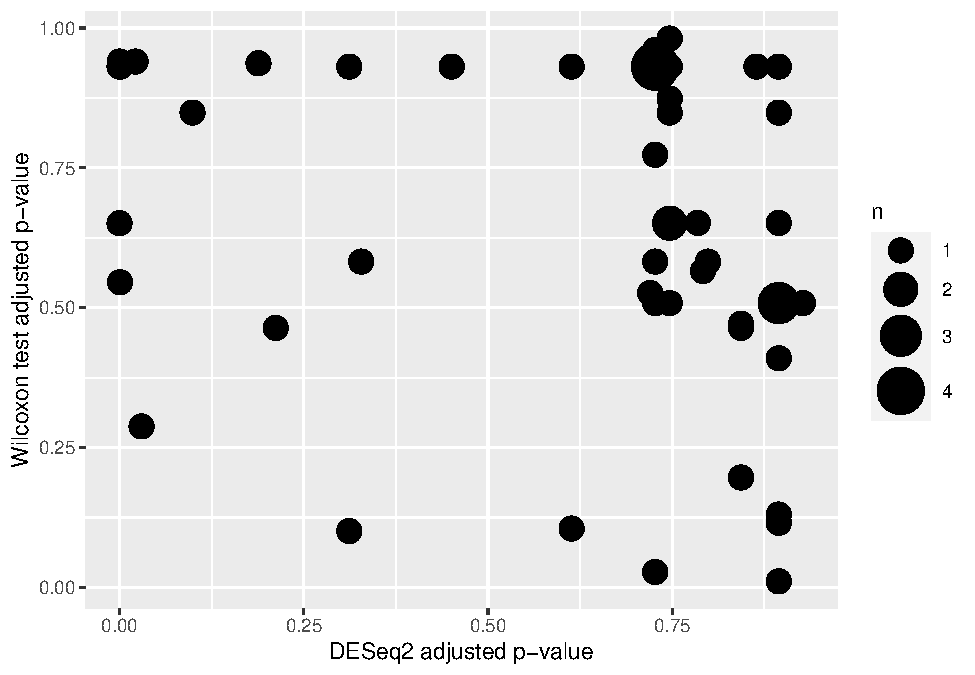
\includegraphics{radboud2021_material_files/figure-latex/unnamed-chunk-33-1.pdf}

Prints number of p-values under 0.05

\begin{Shaded}
\begin{Highlighting}[]
\FunctionTok{print}\NormalTok{(}\FunctionTok{paste0}\NormalTok{(}\StringTok{"DESeq2 p{-}values under 0.05: "}\NormalTok{, }
             \FunctionTok{sum}\NormalTok{(df}\SpecialCharTok{$}\NormalTok{padj}\SpecialCharTok{\textless{}}\FloatTok{0.05}\NormalTok{, }\AttributeTok{na.rm =} \ConstantTok{TRUE}\NormalTok{), }\StringTok{"/"}\NormalTok{, }\FunctionTok{length}\NormalTok{(df}\SpecialCharTok{$}\NormalTok{padj)))}
\end{Highlighting}
\end{Shaded}

\begin{verbatim}
## [1] "DESeq2 p-values under 0.05: 7/54"
\end{verbatim}

\begin{Shaded}
\begin{Highlighting}[]
\FunctionTok{print}\NormalTok{(}\FunctionTok{paste0}\NormalTok{(}\StringTok{"Wilcoxon test p{-}values under 0.05: "}\NormalTok{, }
             \FunctionTok{sum}\NormalTok{(wilcoxon\_p}\SpecialCharTok{$}\NormalTok{p\_adjusted}\SpecialCharTok{\textless{}}\FloatTok{0.05}\NormalTok{, }\AttributeTok{na.rm =} \ConstantTok{TRUE}\NormalTok{), }\StringTok{"/"}\NormalTok{, }
             \FunctionTok{length}\NormalTok{(wilcoxon\_p}\SpecialCharTok{$}\NormalTok{p\_adjusted)))}
\end{Highlighting}
\end{Shaded}

\begin{verbatim}
## [1] "Wilcoxon test p-values under 0.05: 2/54"
\end{verbatim}

\hypertarget{comparison-of-abundance}{%
\section{Comparison of abundance}\label{comparison-of-abundance}}

In previous steps, we got information which taxa vary between ADHD and control groups.
Let's plot those taxa in the boxplot, and compare visually if abundances of those taxa
differ in ADHD and control samples. For comparison, let's plot also taxa that do not
differ between ADHD and control groups.

Let's first gather data about taxa that have highest p-values.

\begin{Shaded}
\begin{Highlighting}[]
\CommentTok{\# There are some taxa that do not include Genus level information. They are}
\CommentTok{\# excluded from analysis.}
\CommentTok{\# str\_detect finds if the pattern is present in values of "taxon" column.}
\CommentTok{\# Subset is taken, only those rows are included that do not include the pattern.}
\NormalTok{df }\OtherTok{\textless{}{-}}\NormalTok{ df[ }\SpecialCharTok{!}\NormalTok{stringr}\SpecialCharTok{::}\FunctionTok{str\_detect}\NormalTok{(df}\SpecialCharTok{$}\NormalTok{taxon, }\StringTok{"Genus:uncultured"}\NormalTok{), ]}

\CommentTok{\# Sorts p{-}values in decreasing order. Takes 3rd first ones. Takes those rows that match}
\CommentTok{\# with p{-}values. Takes taxa. }
\NormalTok{highest3 }\OtherTok{\textless{}{-}}\NormalTok{ df[df}\SpecialCharTok{$}\NormalTok{padj }\SpecialCharTok{\%in\%} \FunctionTok{sort}\NormalTok{(df}\SpecialCharTok{$}\NormalTok{padj, }\AttributeTok{decreasing =} \ConstantTok{TRUE}\NormalTok{)[}\DecValTok{1}\SpecialCharTok{:}\DecValTok{3}\NormalTok{], ]}\SpecialCharTok{$}\NormalTok{taxon}

\CommentTok{\# From clr transformed table, takes only those taxa that had highest p{-}values}
\NormalTok{highest3 }\OtherTok{\textless{}{-}} \FunctionTok{assay}\NormalTok{(tse\_genus, }\StringTok{"clr"}\NormalTok{)[highest3, ]}

\CommentTok{\# Transposes the table}
\NormalTok{highest3 }\OtherTok{\textless{}{-}} \FunctionTok{t}\NormalTok{(highest3)}

\CommentTok{\# Adds colData that includes patient status infomation}
\NormalTok{highest3 }\OtherTok{\textless{}{-}} \FunctionTok{data.frame}\NormalTok{(highest3, }\FunctionTok{as.data.frame}\NormalTok{(}\FunctionTok{colData}\NormalTok{(tse\_genus)))}

\CommentTok{\# Some taxa names are that long that they don\textquotesingle{}t fit nicely into title. }
\CommentTok{\# So let\textquotesingle{}s add there a line break after e.g. "Genus". }
\CommentTok{\# Here the dot after e.g. Genus is replaced with ": \textbackslash{}n"}
\FunctionTok{colnames}\NormalTok{(highest3)[}\DecValTok{1}\SpecialCharTok{:}\DecValTok{3}\NormalTok{] }\OtherTok{\textless{}{-}} \FunctionTok{lapply}\NormalTok{(}\FunctionTok{colnames}\NormalTok{(highest3)[}\DecValTok{1}\SpecialCharTok{:}\DecValTok{3}\NormalTok{], }\ControlFlowTok{function}\NormalTok{(x)\{}
  \CommentTok{\# Replaces the first dot}
\NormalTok{  temp }\OtherTok{\textless{}{-}}\NormalTok{ stringr}\SpecialCharTok{::}\FunctionTok{str\_replace}\NormalTok{(x, }\StringTok{"[.]"}\NormalTok{, }\StringTok{": "}\NormalTok{)}
  
  \CommentTok{\# Replace all other dots and underscores with space}
\NormalTok{  temp }\OtherTok{\textless{}{-}}\NormalTok{ stringr}\SpecialCharTok{::}\FunctionTok{str\_replace\_all}\NormalTok{(temp, }\FunctionTok{c}\NormalTok{(}\StringTok{"[.]"} \OtherTok{=} \StringTok{" "}\NormalTok{, }\StringTok{"\_"} \OtherTok{=} \StringTok{" "}\NormalTok{))}
  
  \CommentTok{\# Adds line break so that 25 characters is the maximal width}
\NormalTok{  temp }\OtherTok{\textless{}{-}}\NormalTok{ stringr}\SpecialCharTok{::}\FunctionTok{str\_wrap}\NormalTok{(temp, }\AttributeTok{width =} \DecValTok{25}\NormalTok{)}
\NormalTok{\})}
\end{Highlighting}
\end{Shaded}

Next, let's do the same but for taxa with lowest p-values.

\begin{Shaded}
\begin{Highlighting}[]
\CommentTok{\# Sorts p{-}values in increasing order. Takes 3rd first ones. }
\CommentTok{\# Takes those rows that match with p{-}values. Takes taxa. }
\NormalTok{lowest3 }\OtherTok{\textless{}{-}}\NormalTok{ df[df}\SpecialCharTok{$}\NormalTok{padj }\SpecialCharTok{\%in\%} \FunctionTok{sort}\NormalTok{(df}\SpecialCharTok{$}\NormalTok{padj, }\AttributeTok{decreasing =} \ConstantTok{FALSE}\NormalTok{)[}\DecValTok{1}\SpecialCharTok{:}\DecValTok{3}\NormalTok{], ]}\SpecialCharTok{$}\NormalTok{taxon}

\CommentTok{\# From clr transformed table, takes only those taxa that had lowest p{-}values}
\NormalTok{lowest3 }\OtherTok{\textless{}{-}}\FunctionTok{assay}\NormalTok{(tse\_genus, }\StringTok{"clr"}\NormalTok{)[lowest3, ]}

\CommentTok{\# Transposes the table}
\NormalTok{lowest3 }\OtherTok{\textless{}{-}} \FunctionTok{t}\NormalTok{(lowest3)}

\CommentTok{\# Adds colData that includes patient status infomation}
\NormalTok{lowest3 }\OtherTok{\textless{}{-}} \FunctionTok{data.frame}\NormalTok{(lowest3, }\FunctionTok{as.data.frame}\NormalTok{(}\FunctionTok{colData}\NormalTok{(tse\_genus)))}

\CommentTok{\# Some taxa names are that long that they don\textquotesingle{}t fit nicely into title. }
\CommentTok{\# So let\textquotesingle{}s add there a line break after e.g. "Genus". }
\CommentTok{\# Here the dot after e.g. Genus is replaced with ": \textbackslash{}n"}
\FunctionTok{colnames}\NormalTok{(lowest3)[}\DecValTok{1}\SpecialCharTok{:}\DecValTok{3}\NormalTok{] }\OtherTok{\textless{}{-}} \FunctionTok{lapply}\NormalTok{(}\FunctionTok{colnames}\NormalTok{(lowest3)[}\DecValTok{1}\SpecialCharTok{:}\DecValTok{3}\NormalTok{], }\ControlFlowTok{function}\NormalTok{(x)\{}
  \CommentTok{\# Replaces the first dot}
\NormalTok{  temp }\OtherTok{\textless{}{-}}\NormalTok{ stringr}\SpecialCharTok{::}\FunctionTok{str\_replace}\NormalTok{(x, }\StringTok{"[.]"}\NormalTok{, }\StringTok{": "}\NormalTok{)}
  
  \CommentTok{\# Replace all other dots and underscores with space}
\NormalTok{  temp }\OtherTok{\textless{}{-}}\NormalTok{ stringr}\SpecialCharTok{::}\FunctionTok{str\_replace\_all}\NormalTok{(temp, }\FunctionTok{c}\NormalTok{(}\StringTok{"[.]"} \OtherTok{=} \StringTok{" "}\NormalTok{, }\StringTok{"\_"} \OtherTok{=} \StringTok{" "}\NormalTok{))}
  
  \CommentTok{\# Adds line break so that 25 characters is the maximal width}
\NormalTok{  temp }\OtherTok{\textless{}{-}}\NormalTok{ stringr}\SpecialCharTok{::}\FunctionTok{str\_wrap}\NormalTok{(temp, }\AttributeTok{width =} \DecValTok{25}\NormalTok{)}
\NormalTok{\})}
\end{Highlighting}
\end{Shaded}

Then we can plot these six different taxa. Let's arrange them into the same picture.

\begin{Shaded}
\begin{Highlighting}[]
\CommentTok{\# Puts plots in the same picture}
\NormalTok{gridExtra}\SpecialCharTok{::}\FunctionTok{grid.arrange}\NormalTok{(}
  
  \CommentTok{\# Plot 1}
  \FunctionTok{ggplot}\NormalTok{(highest3, }\FunctionTok{aes}\NormalTok{(}\AttributeTok{x =}\NormalTok{ patient\_status, }\AttributeTok{y =}\NormalTok{ highest3[,}\DecValTok{1}\NormalTok{])) }\SpecialCharTok{+} 
    \FunctionTok{geom\_boxplot}\NormalTok{() }\SpecialCharTok{+} 
    \FunctionTok{ylab}\NormalTok{(}\StringTok{"CLR abundances"}\NormalTok{) }\SpecialCharTok{+} \CommentTok{\# y axis title}
    \FunctionTok{ggtitle}\NormalTok{(}\FunctionTok{names}\NormalTok{(highest3)[}\DecValTok{1}\NormalTok{]) }\SpecialCharTok{+} \CommentTok{\# main title}
    \FunctionTok{theme}\NormalTok{(}\AttributeTok{title =} \FunctionTok{element\_text}\NormalTok{(}\AttributeTok{size =} \DecValTok{7}\NormalTok{),}
          \AttributeTok{axis.text =} \FunctionTok{element\_text}\NormalTok{(}\AttributeTok{size =} \DecValTok{7}\NormalTok{),}
          \AttributeTok{axis.title.x=}\FunctionTok{element\_blank}\NormalTok{()), }\CommentTok{\# makes titles smaller, removes x axis title}
  
  \CommentTok{\# Plot 2}
  \FunctionTok{ggplot}\NormalTok{(highest3, }\FunctionTok{aes}\NormalTok{(}\AttributeTok{x =}\NormalTok{ patient\_status, }\AttributeTok{y =}\NormalTok{ highest3[,}\DecValTok{2}\NormalTok{])) }\SpecialCharTok{+} 
    \FunctionTok{geom\_boxplot}\NormalTok{() }\SpecialCharTok{+} 
    \FunctionTok{ylab}\NormalTok{(}\StringTok{"CLR abundances"}\NormalTok{) }\SpecialCharTok{+} \CommentTok{\# y axis title}
    \FunctionTok{ggtitle}\NormalTok{(}\FunctionTok{names}\NormalTok{(highest3)[}\DecValTok{2}\NormalTok{]) }\SpecialCharTok{+} \CommentTok{\# main title}
    \FunctionTok{theme}\NormalTok{(}\AttributeTok{title =} \FunctionTok{element\_text}\NormalTok{(}\AttributeTok{size =} \DecValTok{7}\NormalTok{),}
          \AttributeTok{axis.text =} \FunctionTok{element\_text}\NormalTok{(}\AttributeTok{size =} \DecValTok{7}\NormalTok{),}
          \AttributeTok{axis.title.x=}\FunctionTok{element\_blank}\NormalTok{()), }\CommentTok{\# makes titles smaller, removes x axis title}
  
  \CommentTok{\# Plot 3}
  \FunctionTok{ggplot}\NormalTok{(highest3, }\FunctionTok{aes}\NormalTok{(}\AttributeTok{x =}\NormalTok{ patient\_status, }\AttributeTok{y =}\NormalTok{ highest3[,}\DecValTok{3}\NormalTok{])) }\SpecialCharTok{+} 
    \FunctionTok{geom\_boxplot}\NormalTok{() }\SpecialCharTok{+} 
    \FunctionTok{ylab}\NormalTok{(}\StringTok{"CLR abundances"}\NormalTok{) }\SpecialCharTok{+} \CommentTok{\# y axis title}
    \FunctionTok{ggtitle}\NormalTok{(}\FunctionTok{names}\NormalTok{(highest3)[}\DecValTok{3}\NormalTok{]) }\SpecialCharTok{+} \CommentTok{\# main title}
    \FunctionTok{theme}\NormalTok{(}\AttributeTok{title =} \FunctionTok{element\_text}\NormalTok{(}\AttributeTok{size =} \DecValTok{7}\NormalTok{),}
          \AttributeTok{axis.text =} \FunctionTok{element\_text}\NormalTok{(}\AttributeTok{size =} \DecValTok{7}\NormalTok{),}
          \AttributeTok{axis.title.x=}\FunctionTok{element\_blank}\NormalTok{()), }\CommentTok{\# makes titles smaller, removes x axis title}
  
  \CommentTok{\# Plot 4}
  \FunctionTok{ggplot}\NormalTok{(lowest3, }\FunctionTok{aes}\NormalTok{(}\AttributeTok{x =}\NormalTok{ patient\_status, }\AttributeTok{y =}\NormalTok{ lowest3[,}\DecValTok{1}\NormalTok{])) }\SpecialCharTok{+} 
    \FunctionTok{geom\_boxplot}\NormalTok{() }\SpecialCharTok{+} 
    \FunctionTok{ylab}\NormalTok{(}\StringTok{"CLR abundances"}\NormalTok{) }\SpecialCharTok{+} \CommentTok{\# y axis title}
    \FunctionTok{ggtitle}\NormalTok{(}\FunctionTok{names}\NormalTok{(lowest3)[}\DecValTok{1}\NormalTok{]) }\SpecialCharTok{+} \CommentTok{\# main title}
    \FunctionTok{theme}\NormalTok{(}\AttributeTok{title =} \FunctionTok{element\_text}\NormalTok{(}\AttributeTok{size =} \DecValTok{7}\NormalTok{),}
          \AttributeTok{axis.text =} \FunctionTok{element\_text}\NormalTok{(}\AttributeTok{size =} \DecValTok{7}\NormalTok{),}
          \AttributeTok{axis.title.x=}\FunctionTok{element\_blank}\NormalTok{()), }\CommentTok{\# makes titles smaller, removes x axis title}
  
  \CommentTok{\# Plot 5}
  \FunctionTok{ggplot}\NormalTok{(lowest3, }\FunctionTok{aes}\NormalTok{(}\AttributeTok{x =}\NormalTok{ patient\_status, }\AttributeTok{y =}\NormalTok{ lowest3[,}\DecValTok{2}\NormalTok{])) }\SpecialCharTok{+} 
    \FunctionTok{geom\_boxplot}\NormalTok{() }\SpecialCharTok{+} 
    \FunctionTok{ylab}\NormalTok{(}\StringTok{"CLR abundances"}\NormalTok{) }\SpecialCharTok{+} \CommentTok{\# y axis title}
    \FunctionTok{ggtitle}\NormalTok{(}\FunctionTok{names}\NormalTok{(lowest3)[}\DecValTok{2}\NormalTok{]) }\SpecialCharTok{+} \CommentTok{\# main title}
    \FunctionTok{theme}\NormalTok{(}\AttributeTok{title =} \FunctionTok{element\_text}\NormalTok{(}\AttributeTok{size =} \DecValTok{7}\NormalTok{),}
          \AttributeTok{axis.text =} \FunctionTok{element\_text}\NormalTok{(}\AttributeTok{size =} \DecValTok{7}\NormalTok{),}
          \AttributeTok{axis.title.x=}\FunctionTok{element\_blank}\NormalTok{()), }\CommentTok{\# makes titles smaller, removes x axis title}
  
  \CommentTok{\# Plot 6}
  \FunctionTok{ggplot}\NormalTok{(lowest3, }\FunctionTok{aes}\NormalTok{(}\AttributeTok{x =}\NormalTok{ patient\_status, }\AttributeTok{y =}\NormalTok{ lowest3[,}\DecValTok{3}\NormalTok{])) }\SpecialCharTok{+} 
    \FunctionTok{geom\_boxplot}\NormalTok{() }\SpecialCharTok{+} 
    \FunctionTok{ylab}\NormalTok{(}\StringTok{"CLR abundances"}\NormalTok{) }\SpecialCharTok{+} \CommentTok{\# y axis title}
    \FunctionTok{ggtitle}\NormalTok{(}\FunctionTok{names}\NormalTok{(lowest3)[}\DecValTok{3}\NormalTok{]) }\SpecialCharTok{+} \CommentTok{\# main title}
    \FunctionTok{theme}\NormalTok{(}\AttributeTok{title =} \FunctionTok{element\_text}\NormalTok{(}\AttributeTok{size =} \DecValTok{7}\NormalTok{),}
          \AttributeTok{axis.text =} \FunctionTok{element\_text}\NormalTok{(}\AttributeTok{size =} \DecValTok{7}\NormalTok{),}
          \AttributeTok{axis.title.x=}\FunctionTok{element\_blank}\NormalTok{()), }\CommentTok{\# makes titles smaller, removes x axis title}
  
  \CommentTok{\# 3 columns and 2 rows}
  \AttributeTok{ncol =} \DecValTok{3}\NormalTok{, }
  \AttributeTok{nrow =} \DecValTok{2}
\NormalTok{)}
\end{Highlighting}
\end{Shaded}

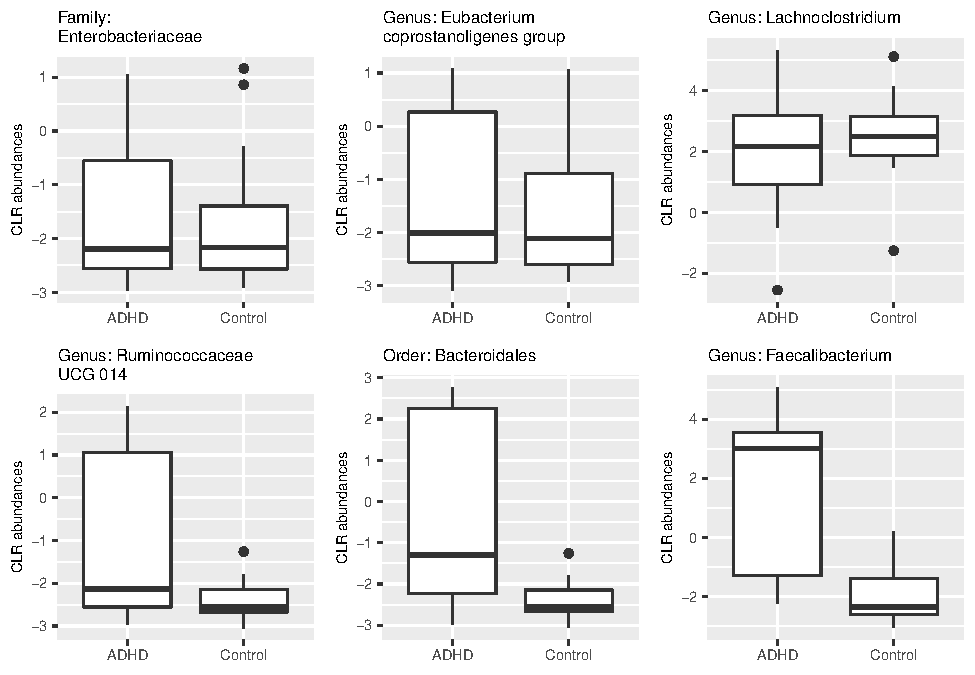
\includegraphics{radboud2021_material_files/figure-latex/unnamed-chunk-37-1.pdf}

\hypertarget{study-material}{%
\chapter{Study material}\label{study-material}}

\hypertarget{lecture-slides}{%
\section{Lecture slides}\label{lecture-slides}}

To be added.

\hypertarget{example-solutions-1}{%
\section{Example solutions}\label{example-solutions-1}}

To be added.

\hypertarget{r-programming-resources}{%
\section{R programming resources}\label{r-programming-resources}}

\begin{itemize}
\tightlist
\item
  R programming basics: \href{https://www.rstudio.com/wp-content/uploads/2016/10/r-cheat-sheet-3.pdf}{Base R}
\item
  Basics of R programming: \href{https://raw.githubusercontent.com/rstudio/cheatsheets/master/base-r.pdf}{Base R}
\item
  \href{https://www.rstudio.com/resources/cheatsheets/}{R cheat sheets}
\item
  R visualization with \href{https://www.rstudio.com/wp-content/uploads/2016/11/ggplot2-cheatsheet-2.1.pdf}{ggplot2}
\item
  \href{http://www.cookbook-r.com/Graphs/}{R graphics cookbook}
\end{itemize}

Rmarkdown

\begin{itemize}
\tightlist
\item
  \href{https://rmarkdown.rstudio.com/}{Rmarkdown tips}
\end{itemize}

RStudio

\begin{itemize}
\tightlist
\item
  \href{https://www.rstudio.com/wp-content/uploads/2016/01/rstudio-IDE-cheatsheet.pdf}{RStudio cheat sheet}
\end{itemize}

\hypertarget{resources-for-treesummarizedexperiment}{%
\section{Resources for TreeSummarizedExperiment}\label{resources-for-treesummarizedexperiment}}

\begin{itemize}
\tightlist
\item
  SingleCellExperiment

  \begin{itemize}
  \tightlist
  \item
    \href{https://bioconductor.org/packages/release/bioc/vignettes/SingleCellExperiment/inst/doc/intro.html}{Publication}
  \item
    \href{https://bioconductor.org/packages/release/bioc/html/SingleCellExperiment.html}{Project page}
  \end{itemize}
\item
  SummarizedExperiment

  \begin{itemize}
  \tightlist
  \item
    \href{https://bioconductor.org/packages/release/bioc/vignettes/SummarizedExperiment/inst/doc/SummarizedExperiment.html}{Publication}
  \item
    \href{https://bioconductor.org/packages/release/bioc/html/SummarizedExperiment.html}{Project page}
  \end{itemize}
\item
  TreeSummarizedExperiment

  \begin{itemize}
  \tightlist
  \item
    \href{https://f1000research.com/articles/9-1246}{Publication}
  \item
    \href{https://www.bioconductor.org/packages/release/bioc/html/TreeSummarizedExperiment.html}{Project page}
  \end{itemize}
\end{itemize}

\hypertarget{resources-for-phyloseq}{%
\section{Resources for phyloseq}\label{resources-for-phyloseq}}

\begin{itemize}
\tightlist
\item
  \href{https://microsud.github.io/Tools-Microbiome-Analysis/}{List of R tools for microbiome analysis}
\item
  \href{http://journals.plos.org/plosone/article?id=10.1371/journal.pone.0061217}{phyloseq}
\item
  \href{http://microbiome.github.io/tutorials/}{microbiome tutorial}
\item
  \href{https://microsud.github.io/microbiomeutilities/}{microbiomeutilities}
\item
  Bioconductor Workflow for Microbiome Data Analysis: from raw reads to community analyses (\href{https://f1000research.com/articles/5-1492/v2}{Callahan et al.~F1000, 2016}).
\end{itemize}

\hypertarget{further-reading}{%
\section{Further reading}\label{further-reading}}

\begin{itemize}
\item
  \href{https://datacarpentry.org/R-ecology-lesson/}{Data Analysis and Visualization in R for Ecologists} by Data Carpentry
\item
  \href{http://web.stanford.edu/class/bios221/book/}{Modern Statistics for Modern Biology. Holmes \& Huber (2018)} for background in statistical analysis
\item
  \href{https://openresearchlabs.github.io/publications/papers/2018-Shetty-Lahti-MDS.pdf}{Microbiome Data Science. Shetty \& Lahti, 2019}
\end{itemize}

\hypertarget{miscellaneous-material}{%
\chapter{Miscellaneous material}\label{miscellaneous-material}}

\hypertarget{shapiro-wilk-test}{%
\section{Shapiro-Wilk test}\label{shapiro-wilk-test}}

If necessary, it is possible to assess normality of the data with Shapiro-Wilk test.

\begin{Shaded}
\begin{Highlighting}[]
\CommentTok{\# Does Shapiro{-}Wilk test. Does it only for columns that contain abundances, not for}
\CommentTok{\# column that contain Groups.}

\NormalTok{normality\_test\_p }\OtherTok{\textless{}{-}} \FunctionTok{c}\NormalTok{()}

\ControlFlowTok{for}\NormalTok{ (column }\ControlFlowTok{in} 
\NormalTok{     abundance\_analysis\_data[, }\SpecialCharTok{!}\FunctionTok{names}\NormalTok{(abundance\_analysis\_data) }\SpecialCharTok{\%in\%} \StringTok{"patient\_status"}\NormalTok{])\{}
  \CommentTok{\# Does Shapiro{-}Wilk test}
\NormalTok{  result }\OtherTok{\textless{}{-}} \FunctionTok{shapiro.test}\NormalTok{(column)}
  
  \CommentTok{\# Stores p{-}value to vector}
\NormalTok{  normality\_test\_p }\OtherTok{\textless{}{-}} \FunctionTok{c}\NormalTok{(normality\_test\_p, result}\SpecialCharTok{$}\NormalTok{p.value)}
\NormalTok{\}}

\FunctionTok{print}\NormalTok{(}\FunctionTok{paste0}\NormalTok{(}\StringTok{"P{-}values over 0.05: "}\NormalTok{, }\FunctionTok{sum}\NormalTok{(normality\_test\_p}\SpecialCharTok{\textgreater{}}\FloatTok{0.05}\NormalTok{), }\StringTok{"/"}\NormalTok{, }
             \FunctionTok{length}\NormalTok{(normality\_test\_p)))}
\end{Highlighting}
\end{Shaded}

\begin{verbatim}
## [1] "P-values over 0.05: 7/54"
\end{verbatim}

\hypertarget{deseq-details}{%
\section{Deseq details}\label{deseq-details}}

\begin{enumerate}
\def\labelenumi{\arabic{enumi}.}
\tightlist
\item
  Raw counts are normalized by log-based scaling.\\
\item
  Taxa-wise variance is estimated. These values tell how much each taxa varies between samples.\\
\item
  A curve is fitted over all those taxa-wise variance estimates that we got in the last step.\\
  This model tells how big the variance is in a specific abundance level.
\item
  The model is used to shrink those individual variance estimates to avoid the effect of,
  e.g., small sample size and higher variance. This reduces the likelihood to get
  false positives.\\
\item
  Variance estimates are used to compare different groups. We receive a result that shows whether the variance is explained by groups.
\end{enumerate}

\hypertarget{exercise-solutions}{%
\chapter{Exercise Solutions}\label{exercise-solutions}}

This section includes exemplary solutions to the exercises presented earlier.

\hypertarget{section-5}{%
\section{Section 5}\label{section-5}}

Link:

\begin{itemize}
\tightlist
\item
  \href{import.Rmd}{Rmd}
\end{itemize}

\hypertarget{section-6}{%
\section{Section 6}\label{section-6}}

Links:

\begin{itemize}
\item
  \href{06-3-ex-sol-ADHD.Rmd}{Rmd}
\item
  \href{06-3-ex-sol-ADHD.html}{HTML}
\end{itemize}

\hypertarget{section-7}{%
\section{Section 7}\label{section-7}}

Links:

\begin{itemize}
\item
  \href{07-3-ex-sol-ADHD.Rmd}{Rmd}
\item
  \href{07-3-ex-sol-ADHD.html}{HTML}
\end{itemize}

\hypertarget{section-8}{%
\section{Section 8}\label{section-8}}

Links:

\begin{itemize}
\item
  \href{08-5-ex-sol-ADHD.Rmd}{Rmd}
\item
  \href{08-5-ex-sol-ADHD.html}{HTML}
\end{itemize}

\end{document}
